% Options for packages loaded elsewhere
\PassOptionsToPackage{unicode}{hyperref}
\PassOptionsToPackage{hyphens}{url}
%
\documentclass[
]{article}
\usepackage{amsmath,amssymb}
\usepackage{iftex}
\ifPDFTeX
  \usepackage[T1]{fontenc}
  \usepackage[utf8]{inputenc}
  \usepackage{textcomp} % provide euro and other symbols
\else % if luatex or xetex
  \usepackage{unicode-math} % this also loads fontspec
  \defaultfontfeatures{Scale=MatchLowercase}
  \defaultfontfeatures[\rmfamily]{Ligatures=TeX,Scale=1}
\fi
\usepackage{lmodern}
\ifPDFTeX\else
  % xetex/luatex font selection
\fi
% Use upquote if available, for straight quotes in verbatim environments
\IfFileExists{upquote.sty}{\usepackage{upquote}}{}
\IfFileExists{microtype.sty}{% use microtype if available
  \usepackage[]{microtype}
  \UseMicrotypeSet[protrusion]{basicmath} % disable protrusion for tt fonts
}{}
\makeatletter
\@ifundefined{KOMAClassName}{% if non-KOMA class
  \IfFileExists{parskip.sty}{%
    \usepackage{parskip}
  }{% else
    \setlength{\parindent}{0pt}
    \setlength{\parskip}{6pt plus 2pt minus 1pt}}
}{% if KOMA class
  \KOMAoptions{parskip=half}}
\makeatother
\usepackage{xcolor}
\usepackage[margin=1in]{geometry}
\usepackage{longtable,booktabs,array}
\usepackage{calc} % for calculating minipage widths
% Correct order of tables after \paragraph or \subparagraph
\usepackage{etoolbox}
\makeatletter
\patchcmd\longtable{\par}{\if@noskipsec\mbox{}\fi\par}{}{}
\makeatother
% Allow footnotes in longtable head/foot
\IfFileExists{footnotehyper.sty}{\usepackage{footnotehyper}}{\usepackage{footnote}}
\makesavenoteenv{longtable}
\usepackage{graphicx}
\makeatletter
\def\maxwidth{\ifdim\Gin@nat@width>\linewidth\linewidth\else\Gin@nat@width\fi}
\def\maxheight{\ifdim\Gin@nat@height>\textheight\textheight\else\Gin@nat@height\fi}
\makeatother
% Scale images if necessary, so that they will not overflow the page
% margins by default, and it is still possible to overwrite the defaults
% using explicit options in \includegraphics[width, height, ...]{}
\setkeys{Gin}{width=\maxwidth,height=\maxheight,keepaspectratio}
% Set default figure placement to htbp
\makeatletter
\def\fps@figure{htbp}
\makeatother
\setlength{\emergencystretch}{3em} % prevent overfull lines
\providecommand{\tightlist}{%
  \setlength{\itemsep}{0pt}\setlength{\parskip}{0pt}}
\setcounter{secnumdepth}{5}
\usepackage{amsmath}
\usepackage{tikz}
\usepackage{pgfplots}
\usepackage{caption}
\usepackage{subcaption}
\usepackage{cancel}
\usepackage{mathtools}
\usepackage{annotate-equations}
\ifLuaTeX
  \usepackage{selnolig}  % disable illegal ligatures
\fi
\IfFileExists{bookmark.sty}{\usepackage{bookmark}}{\usepackage{hyperref}}
\IfFileExists{xurl.sty}{\usepackage{xurl}}{} % add URL line breaks if available
\urlstyle{same}
\hypersetup{
  pdftitle={Notas de Aulas - MI401},
  pdfauthor={Caio Gomes Alves},
  hidelinks,
  pdfcreator={LaTeX via pandoc}}

\title{Notas de Aulas - MI401}
\usepackage{etoolbox}
\makeatletter
\providecommand{\subtitle}[1]{% add subtitle to \maketitle
  \apptocmd{\@title}{\par {\large #1 \par}}{}{}
}
\makeatother
\subtitle{Probabilidade}
\author{Caio Gomes Alves}
\date{03/2025}

\usepackage{amsthm}
\newtheorem{theorem}{Theorem}[section]
\newtheorem{lemma}{Lemma}[section]
\newtheorem{corollary}{Corollary}[section]
\newtheorem{proposition}{Proposition}[section]
\newtheorem{conjecture}{Conjecture}[section]
\theoremstyle{definition}
\newtheorem{definition}{Definition}[section]
\theoremstyle{definition}
\newtheorem{example}{Example}[section]
\theoremstyle{definition}
\newtheorem{exercise}{Exercise}[section]
\theoremstyle{definition}
\newtheorem{hypothesis}{Hypothesis}[section]
\theoremstyle{remark}
\newtheorem*{remark}{Remark}
\newtheorem*{solution}{Solution}
\begin{document}
\maketitle

\renewcommand*\contentsname{Conteúdos}
{
\setcounter{tocdepth}{2}
\tableofcontents
}
\newpage

\hypertarget{prefuxe1cio}{%
\section{Prefácio}\label{prefuxe1cio}}

Este ``livro'' consiste de notas de aulas da matéria MI401 - Probabilidade, do Programa de Mestrado em Estatística, do Instituto de Matemática, Estatística e Computação Científica (IMECC), da Universidade Estadual de Campinas - UNICAMP.

Os seus conteúdos são baseados nas notas tomadas durante as aulas e o livro ``Probabilidade: um curso em nível intermediário'', do autor Barry R. James, 5ª edição.

\newpage

\hypertarget{definiuxe7uxf5es-buxe1sicas}{%
\section{Definições Básicas}\label{definiuxe7uxf5es-buxe1sicas}}

\hypertarget{modelo-probabiluxedstico}{%
\subsection{Modelo Probabilístico}\label{modelo-probabiluxedstico}}

Suponha que é realizado um experimento ``sob certas condições'', sendo \textbf{\(\Omega\)} o conjunto de resultados possíveis do experimento (também chamado de resultados elementares). Chamamos \textbf{\(\Omega\)} de \textbf{espaço amostral do experimento}, com a representação axiomática sendo dada por: \(\Omega = \{\omega : \omega \in \Omega\}\).

\begin{example}
Considere o lançamento de um dado honesto. Nesse caso, temos que \(\Omega = \{1,2,3,4,5,6\}\), em que cada \(\{i\}\) é um evento elementar, sendo eles \{1\},\{2\},\{3\},\{4\},\{5\} e \{6\}.
\end{example}

Temos então que eventos são coleções de pontos em \(\Omega\), por exemplo um evento \(A = \{2,4,6\}\) (números pares no lançamento de um dado honesto). Assim, temos as seguintes suposições para eventos:

\begin{enumerate}
\def\labelenumi{\arabic{enumi}.}
\tightlist
\item
  Todo resultado possível no experimento corresponde a um e somente um \(\omega \in \Omega\);
\item
  Resultados diferentes correspondem a elementos diferentes em \(\Omega\).
\end{enumerate}

\begin{definition}
Seja um espaço amostral \(\Omega\) de um experimento. Todo subconjunto \(A \subset \Omega\) é um evento. \(\Omega\) é o evento certo e \(\emptyset\) é o evento impossível. Além disso, \(\omega \in \Omega \to \{\omega\}\) é um evento elementar.
\end{definition}

Note-se que, dados \(A\) e \(B\) eventos, tais que \(A \subset \Omega\) e \(B \subset \Omega\), temos que:

\begin{itemize}
\tightlist
\item
  \(A \cup B \to (\omega \in A \text{ e } \omega \notin B)\) ou \((\omega \notin A \text{ e } \omega \in B)\) ou \((\omega \in A \text{ e } \omega \in B)\);
\item
  \(A \cap B \to (\omega \in A \cup \omega \in B)\);
\item
  \(A^{c} \to (\omega \notin A)\);
\item
  \(A \subset B \to\) a ocorrência de \(A\) implica a ocorrência de \(B\);
\item
  \(A \cap B = \emptyset \to\) os eventos \(A\) e \(B\) são mutuamente exclusivos.
\end{itemize}

No campo probabilístico, pensamos em atribuir probabilidades (leia-se chances) a eventos em \(\Omega\).

\begin{definition}[Clássica]
A probabilidade de ocorrência de um evento \(A\), denotada por \(P(A)\) é dada por:

\[P(A) = \frac{\#(A)}{\#(\Omega)} = \frac{\text{nº de resultados favoráveis a }A}{\text{nº de resultados possíveis em }\Omega}\]

Onde \(\#\) indica a cardinalidade de um conjunto (quantidade de elementos no conjunto).
\end{definition}

\begin{example}
Seja \(A = \{2,4,6\}\), os lançamentos pares em um dado honesto. Como \(\Omega = \{1,\dots,6\}\), temos que:

\[P(A) = \frac{3}{6} = \frac{1}{2}\]

Note que o conjunto \(A\) pode ser descrito como a união dos eventos elementares, tais que \(A = \{2\} \cup \{4\} \cup \{6\}\). Nesse caso, podemos ver que a probabilidade de \(A\) não muda, pois:

\begin{align*}
P(\{i\}) &= \frac{\#(\{i\})}{\#(\Omega)} = \frac{1}{6}\\
P(A) &= \frac{\#(\{2\})+\#(\{4\})+\#(\{6\})}{\#(\Omega)} = \frac{1+1+1}{6} = \frac{1}{2}
\end{align*}
\end{example}

\begin{definition}
Um evento \(A\) ao qual atribuímos uma probabilidade é um evento aleatório.
\end{definition}

\hypertarget{uxe1lgebras-de-conjuntos}{%
\subsection{Álgebras de Conjuntos}\label{uxe1lgebras-de-conjuntos}}

Considere o conjunto de eventos em uma família \(\mathcal{A}\) (subconjuntos de \(\Omega\)), de tal modo que \(P:A \to [0,1]\). Uma representação gráfica da relação \(P\) pode ser dada por:

\begin{center}
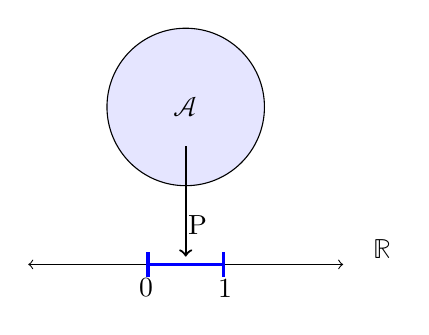
\begin{tikzpicture}
% Desenhando o conjunto A como um círculo:
\draw[fill=blue!10] (0.5,2) circle (1);

% Adicionando o nome do conjunto A:
\node at (0.5,2) {$\mathcal{A}$};

% Desenhando a reta real (-1.5 a 2.5, para ficar simétrico):
\draw[thin, <->] (-1.5,0) -- (2.5,0);
\node at (3, 0.2) {$\mathbb{R}$};

% Desenhando a reta [0,1] de forma a ficar mais aparente:
\draw[|-|, very thick, blue] (0,0) -- (1,0);
\node at (0,-0.3) {$0$};
\node at (1,-0.3) {$1$};

% Desenhando a flecha de A para a reta [0,1]:
\draw[->, thick] (0.5,1.5) -- (0.5,0.1);
\node at (0.65,0.5) {P};
\end{tikzpicture}
\end{center}

\begin{definition}

Seja \(\Omega\) um conjunto não-vazio. Seja \(\mathcal{A}\) uma classe de subconjuntos de \(\Omega\), ela será chamada de \textbf{``Álgebra de subconjuntos de \(\Omega\)''}, caso respeite os seguintes axiomas:

\begin{itemize}
\tightlist
\item
  \(Ax_{1}\) : \(\Omega \in \mathcal{A}\), e definimos \(P(\Omega) = 1\);
\item
  \(Ax_{2}\) : Se \(A \in \mathcal{A} \Rightarrow A^{c} \in \mathcal{A}\), e definimos \(P(A^{c}) = 1 - P(A)\);
\item
  \(Ax_{3}\) : Se \(A \in \mathcal{A}, B \in \mathcal{A} \Rightarrow A \cup B \in \mathcal{A}\).
\end{itemize}

E por consequência desses axiomas, temos as seguintes extensões:

\begin{itemize}
\tightlist
\item
  \(Ax_{4}\) : \(\emptyset \in \mathcal{A}\);
\item
  \(Ax_{5}\) : Sejam \(A_{1}, A_{2}, \dots, A_{n} : A_{i} \in \mathcal{A} \forall i \Rightarrow \bigcup_{i=1}^{n}A_{i} \in \mathcal{A}\) e \(\bigcap_{i = 1}^{n}A_{i} \in \mathcal{A}\).
\end{itemize}

\end{definition}

É fácil verificar a extensão de \(Ax_{4}\) a partir de \(Ax_{1} \text{ e } Ax_{2}\): \(Ax_{1}\) define que \(\Omega \in \mathcal{A}\), e por \(Ax_{2}\) temos que \(\Omega^{c} \in \mathcal{A}\), e por definição temos que \(\Omega^{c} = \emptyset\), logo \(\emptyset \in \mathcal{A}\). Também é interessante notar que, ainda por \(Ax_{2}\), temos que \(P(\emptyset) = 1 - P(\Omega)\), e por \(Ax_{1}\) temos que \(P(\Omega) = 1\), portanto \(P(\emptyset) = 1 - 1 = 0\).

A extensão de \(Ax_{5}\) é dada por indução e pelas Leis de De Morgan: Sejam \(A_{1}, A_{2} \in \mathcal{A}\). Temos pelo axioma \(Ax_{3}\), que \(A_{1} \cup A_{2} \in \mathcal{A}\), podendo assim definir o conjunto \(B = A_{1} \cup A_{2}\), sendo possível ver que \(B \in \mathcal{A}\). Sejam ainda um conjunto \(A_{3} \in \mathcal{A}\), podemos ver que \(B \cup A_{3} \in \mathcal{A}\), e como \(B = A_{1} \cup A_{2}\), temos que \((A_{1} \cup A_{2}) \cup A_{3} \in \mathcal{A}\). Podemos proceder dessa forma para qualquer quantidade (enumerável) de conjuntos, de modo que \(\bigcup_{i = 1}^{n}A_{i} \in \mathcal{A}\). Pelas Leis de De Morgan, sabemos que:

\begin{equation}
\bigcap_{i=1}^{n}A_{i} = \left(\bigcup_{i = 1}^{n}A_{i}^{c}\right)^{c}
\label{eq:demorgan}
\end{equation}

E pela extenção indutiva em \(n\) do axioma \(Ax_{2}\), temos que se \(A_{i}^{c} \in \mathcal{A}, \forall i\), então \(\bigcup_{i = 1}^{n}A_{i}^{c} \in \mathcal{A}\). E como, se um conjunto pertence a \(\mathcal{A}\) seu complementar deve pertencer também, e pelo resultado em \eqref{eq:demorgan}, temos então que:

\begin{equation}
\left(\bigcup_{i = 1}^{n}A_{i}^{c}\right)^{c} = \left(\bigcap_{i = 1}^{n}A_{i}\right) \in \mathcal{A}
\label{eq:axioma5}
\end{equation}

Assim provamos o axioma \(A_{5}\) como extensão indutiva dos axiomas anteriores, indicando que tanto a união quanto a interseção dos \(A_{i}\) pertencem à \(\mathcal{A}\). Podemos também mostrar que a álgebra \(\mathcal{A}\) é fechada também para a operação de diferença entre conjuntos: \(A \in \mathcal{A}, B \in \mathcal{A}, A-B = A \cap B^{c} \in \mathcal{A}\).

\begin{proof}
Considerando que os conjuntos \(A\) e \$B pertencem à \(\mathcal{A}\), podemos utilizar o axioma \(Ax_{2}\) para mostrar que \(A^{c} \in \mathcal{A}\) e \(B^{c} \in \mathcal{A}\). A partir disso, por meio do axioma \(Ax_{5}\) temos que os seguintes conjuntos também pertencem à \(\mathcal{A}\): \(A \cup B, A \cup B^{c}, A^{c} \cup B, A^{c} \cup B^{c}, A \cap B, A \cap B^{c}, A^{c} \cap B, A^{c} \cap B^{c}\). E como temos que \(A \cap B^{c} = A-B\), temos a prova de que \(A-B \in \mathcal{A}\). Além disso, essa prova mostra que a diferença contrária (\(B - A = A^{c} \cap B\)) também pertence à algebra \(\mathcal{A}\).
\end{proof}

Ainda considerando os conjuntos \(A\) e \(B\), existem cinco maneiras como esses conjuntos podem ``interagir'', e podemos mostrar que em todos os casos a diferença \(A-B \in \mathcal{A}\):

\begin{itemize}
\tightlist
\item
  \(A \not\subset B\) e \(A \not\supset B\) e \(A \cap B \neq \emptyset \Rightarrow A-B = A \cap B^{c} \in \mathcal{A}\);
\item
  \(A \not\subset B\) e \(A \not\supset B\) e \(A \cap B = \emptyset \Rightarrow A-B = A \in \mathcal{A}\);
\item
  \(A \supset B \Rightarrow A-B = A \cap B^{c} \in \mathcal{A}\);
\item
  \(A \subset B \Rightarrow A-B = \emptyset \in \mathcal{A}\);
\item
  \(A = B \Rightarrow A-B = \emptyset \in \mathcal{A}\).
\end{itemize}

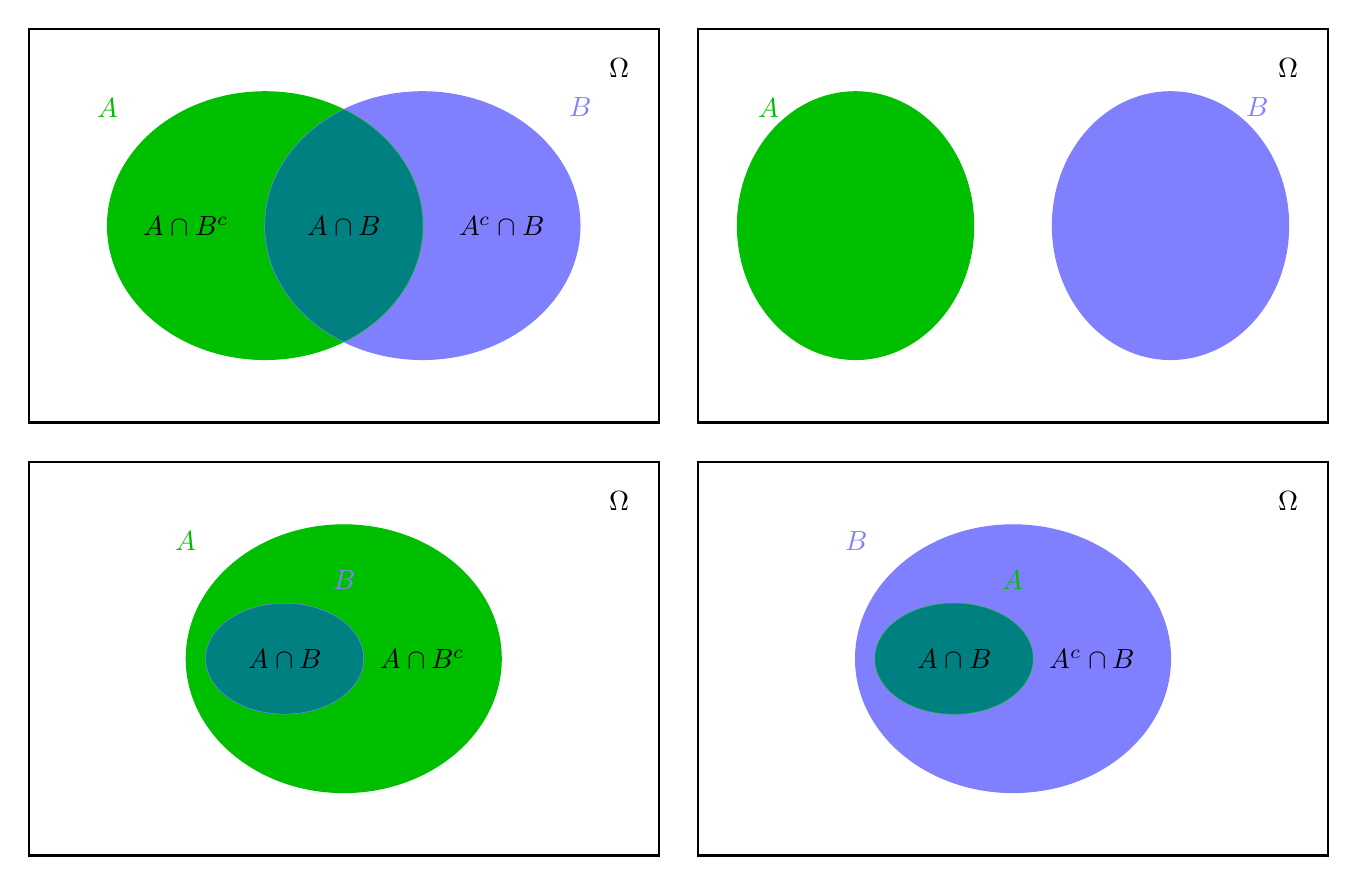
\begin{tikzpicture}
\centering
    % Primeira figura:
    \begin{scope}
    \draw[thick] (0,0) rectangle (8,5);
    \node (n0) at (7.5,4.5) {$\Omega$};
    \def\first{(3,2.5) ellipse (2 cm and 1.7 cm)};
    \def\second{(5,2.5) ellipse (2 cm and 1.7 cm)};
    \fill[fill=green!75!black]\first;
    \fill[fill=blue!50!white]\second;
    \draw[color=green!75!black] \first;
    \draw[color=blue!50!white] \second;
    \begin{scope}
        \clip \first;
        \fill[fill=green!50!blue]\second;
    \end{scope}
    \node (n1) at (1,4) {\textcolor{green!75!black}{$A$}};
    \node (n2) at (7,4) {\textcolor{blue!50!white}{$B$}};
    \node (n3) at (2,2.5) {$A \cap B^{c}$};
    \node (n4) at (6,2.5) {$A^{c} \cap B$};
    \node (n5) at (4,2.5) {$A \cap B$};
    \end{scope}
    % Início da segunda figura:
        \begin{scope}[xshift=8.5cm]
    \draw[thick] (0,0) rectangle (8,5);
    \node (n0) at (7.5,4.5) {$\Omega$};
    \def\first{(2,2.5) ellipse (1.5 cm and 1.7 cm)};
    \def\second{(6,2.5) ellipse (1.5 cm and 1.7 cm)};
    \fill[fill=green!75!black]\first;
    \fill[fill=blue!50!white]\second;
    \draw[color=green!75!black] \first;
    \draw[color=blue!50!white] \second;
    \begin{scope}
        \clip \first;
        \fill[fill=green!50!blue]\second;
    \end{scope}
    \node (n1) at (0.9,4) {\textcolor{green!75!black}{$A$}};
    \node (n2) at (7.1,4) {\textcolor{blue!50!white}{$B$}};
    \end{scope}
    % Início da terceira figura:
    \begin{scope}[yshift=-5.5cm]
    \draw[thick] (0,0) rectangle (8,5);
    \node (n0) at (7.5,4.5) {$\Omega$};
    \def\first{(4,2.5) ellipse (2 cm and 1.7 cm)};
    \def\second{(3.25,2.5) ellipse (1 cm and 0.7 cm)};
    \fill[fill=green!75!black]\first;
    \fill[fill=blue!50!white]\second;
    \draw[color=green!75!black] \first;
    \draw[color=blue!50!white] \second;
    \begin{scope}
        \clip \first;
        \fill[fill=green!50!blue]\second;
    \end{scope}
    \node (n1) at (2,4) {\textcolor{green!75!black}{$A$}};
    \node (n2) at (4,3.5) {\textcolor{blue!50!white}{$B$}};
    \node (n3) at (3.25,2.5) {$A \cap B$};
    \node (n4) at (5,2.5) {$A \cap B^{c}$};
    \end{scope}
    % Início da quarta figura:
    \begin{scope}[xshift=8.5cm,yshift=-5.5cm]
    \draw[thick] (0,0) rectangle (8,5);
    \node (n0) at (7.5,4.5) {$\Omega$};
    \def\first{(4,2.5) ellipse (2 cm and 1.7 cm)};
    \def\second{(3.25,2.5) ellipse (1 cm and 0.7 cm)};
    \fill[fill=blue!50!white]\first;
    \fill[fill=green!75!black]\second;
    \draw[color=blue!50!white] \first;
    \draw[color=green!75!black] \second;
    \begin{scope}
        \clip \first;
        \fill[fill=green!50!blue]\second;
    \end{scope}
    \node (n1) at (2,4) {\textcolor{blue!50!white}{$B$}};
    \node (n2) at (4,3.5) {\textcolor{green!75!black}{$A$}};
    \node (n3) at (3.25,2.5) {$A \cap B$};
    \node (n4) at (5,2.5) {$A^{c} \cap B$};
    \end{scope}
\label{diagramasvenn}
\end{tikzpicture}
\captionof{figure}{Diferentes relações entre $A$ e $B$ demonstradas por Diagramas de Venn. Note que em todos os casos, $A \cap B^{c} \in \mathcal{A}$ ou $A \cap B^{c} = \emptyset \in \mathcal{A} \text{ ou } A \cap B^{c} = A \in \mathcal{A}$}

As representações por Diagramas de Venn apresentadas na figura \ref{diagramasvenn} não é prova formal de que a álgebra \(\mathcal{A}\) é fechada para a diferença, mas é um recurso visual que pode auxiliar no entendimento da relação entre os conjuntos.

\begin{definition}
Uma classe \(\mathcal{A}\) de conjuntos/subconjuntos de \(\Omega \neq \emptyset\), verificando os axiomas \(Ax_{1}, Ax_{2} \text{ e } Ax_{3}\) é chamada de \(\sigma\)-álgebra de subconjuntos de \(\Omega\).
\end{definition}

Note que uma \(\sigma\)-álgebra é sempre uma álgebra. Uma outra forma de construir \(\sigma\)-álgebras é partir de uma álgebra munida dos axiomas de Kolmogorov (Teorema de Carathéodory).

\begin{proposition}
Seja \(\mathcal{A}\) uma \(\sigma\)-álgebra de subconjuntos de \(\Omega\), se \(A_{1}, A_{2},\dots,\) é uma coleção em \(\mathcal{A} \Rightarrow \bigcap_{i=1}^{\infty}A_{n} \in \mathcal{A}\).
\end{proposition}

\begin{example}
\protect\hypertarget{exm:powerset}{}\label{exm:powerset}Seja \(\Omega = \{1,2,3,4,5,6\}\) (o lançamento de um dado cúbico usual). A \(\sigma\)-álgebra usual é definida da seguinte forma e denotada por \(\mathcal{P}(\Omega)\) (chamada de partes de \(\Omega\) ou \emph{powerset} de \(\Omega\)):

\begin{align*}
\mathcal{A} = \{&\emptyset,\{1\},\{2\},\{3\},\{4\},\{5\},\{6\},\\
& \{1,2\},\{1,3\},\{1,4\},\{1,5\},\{1,6\}, \\
&\{2,3\},\{2,4\},\dots,\\
&\Omega\}
\end{align*}
\end{example}

\begin{example}
Definamos a \(\sigma\)-álgebra de Borel no intervalo \(\Omega = [0,1]\). Uma possível definição seria:

\[
\mathcal{A} = \text{ todos os subconjuntos de } [0,1] \text{ cujo cumprimento esteja bem definido}
\]

Podemos, por exemplo, propor uma álgebra para o intervalo \([0,1]\) dada por:

\[
\mathcal{A_{0}} = \{A \subset [0,1]: A \text{ é uma união finita de intervalos }\}
\]

É possível encontrar um conjunto \(A\) tal que \(A \not\in \mathcal{A}\), por exemplo:

\[
A = \left\{\left(0,\frac{1}{2}\right) \cup \left(\frac{1}{2},\frac{3}{4}\right)\cup \dots \cup \left(1-\frac{1}{2^{n}},1-\frac{1}{2^{n+1}}\right)\cup \dots\right\}
\]

Podemos ver que, para qualquer \(n^{*}\) finito, \(\lim_{n \to n^{*}}\left(1 - \frac{1}{2^{n+1}}\right) \neq 1\), de modo que o conjunto \(A\) não cobrirá completamente o intervalo \([0,1]\). Dessa forma, a \(\sigma\)-álgebra de Borel no intervalo \([0,1]\) (denotada \(\mathcal{B}_{[0,1]}\)) é definida como:

\[
\mathcal{B}_{[0,1]} = \left\{A: A \subset [0,1] \text{ e }A \text{ é boreliano}\right\}
\]

Onde boreliano denota que \(A\) é união enumerável (finita ou infinita) de intervalos em \([0,1]\)
\end{example}

\hypertarget{axiomas-de-kolmogorov}{%
\subsection{Axiomas de Kolmogorov}\label{axiomas-de-kolmogorov}}

Seja \(P:\mathcal{A} \rightarrow [0,1]\), com:

\begin{itemize}
\tightlist
\item
  \(Ax_{1}(K): P(A) \ge 0, \forall A \in \mathcal{A}\);
\item
  \(Ax_{2}(K): P(\Omega) = 1\);
\item
  \(Ax_{3}(K):\) Se \(A_{1},A_{2},\dots,A_{n} : A_{i} \in \mathcal{A} \forall i\) e \(A_{i} \cap A_{j} = \emptyset \forall i,j \in \{1,2,\dots,n\}, i \neq j \Rightarrow P\left(\bigcup_{k=1}^{n}A_{k}\right) = \sum_{k=1}^{n}P(A_{k})\).
\end{itemize}

\begin{definition}

Seja \(\Omega\) um conjunto não-vazio, \(\mathcal{A}\) uma \(\sigma\)-álgebra em \(\Omega\), com \(P : \mathcal{A} \to [0,1]\), verificando os axiomas de Kolmogorov, então \(P\) é dita finitamente aditiva. Podemos assim, modificar o axioma \(Ax_{3}(K)\) para:

\begin{itemize}
\tightlist
\item
  \(Ax'_{3}(K):\) Se \(A_{1},A_{2},\dots\) é uma sequência em \(\mathcal{A}\) tal que \(\forall i \neq j, A_{i} \cap A_{j} = \emptyset\), tem-se que \(P\left(\bigcup_{n=1}^{\infty}A_{n}\right) = \sum_{n=1}^{\infty}P(A_{n})\). (\emph{propriedade da \(\sigma\)-aditividade})
\end{itemize}

\end{definition}

\begin{definition}
\(P\) definida em uma \(\sigma\)-álgebra \(\mathcal{A}\), satisfazendo os axiomas de Kolmogorov (\(Ax_{1}(K), Ax_{2}(K), Ax'_{3}(K)\)) é uma medida de probabilidade em \(\mathcal{A}\), constituída pela terna \((\Omega, \mathcal{A},P)\).
\end{definition}

\hypertarget{propriedades-da-medida-de-probabilidade}{%
\subsection{Propriedades da medida de probabilidade}\label{propriedades-da-medida-de-probabilidade}}

\begin{proposition}[Continuidades]
\protect\hypertarget{prp:continuidade}{}\label{prp:continuidade}\leavevmode

\begin{enumerate}
\def\labelenumi{\arabic{enumi}.}
\tightlist
\item
  Seja \(\{A_{i}\}_{i=1}^{\infty}\) uma sequência (crescente) de eventos tais que \(A_{1} \subseteq A_{2} \subseteq A_{3} \subseteq \dots\), e seja \(A = \bigcup_{i=1}^{\infty}A_{i}\), então \(P(A) = \lim_{i \to \infty}P(A_{i})\).
\item
  Seja \(\{B_{i}\}_{i=1}^{\infty}\) uma sequência (decrescente) de eventos tais que \(B_{1} \supseteq B_{2} \supseteq B_{3} \supseteq \dots\), e seja \(B = \bigcap_{i=1}^{\infty}B_{i}\), então \(P(B) = \lim_{i \to \infty}P(B_{i})\).
\end{enumerate}

\end{proposition}

\begin{proof}
\leavevmode

\begin{enumerate}
\def\labelenumi{\arabic{enumi}.}
\tightlist
\item
  Note que, sendo \(A_{0} = \emptyset\), tem-se que \(A = (A_{1} - A_{0}) \cup (A_{2} - A_{1}) \cup (A_{3} - A_{2}) \cup \dots\), ou seja, \(A\) é união disjunta de eventos \(D_{i} = A_{i} - A_{i-1}\), de forma que \(A_{i-1} \subseteq A_{i} \Rightarrow P(A_{i}) = P(A_{i-1}) + P(A_{i} - A_{i-1}) \Rightarrow P(A_{i} - A_{i-1}) = P(A_{i}) - P(A_{i-1})\). Logo, temos que:
\end{enumerate}

\begin{align*}
A = \bigcup_{i=1}^{\infty}D_{i} \xRightarrow{Ax'_{3}(K)} P(A) &= \sum_{i=1}^{\infty}P(D_{i})\\
&= \sum_{i=1}^{\infty}P(A_{i} - A_{i-1})\\
&= \lim_{n \to \infty} \sum_{i=1}^{n} \left[P(A_{i}) - P(A_{i-1})\right] \\
&= \lim_{n \to \infty} \left[P(A_{1}) - P(A_{0}) + P(A_{2}) - P(A_{1}) + P(A_{3}) - P(A_{2}) + \dots\right]\\
&= \lim_{n \to \infty} P(A_{n})
\end{align*}

\begin{enumerate}
\def\labelenumi{\arabic{enumi}.}
\setcounter{enumi}{1}
\tightlist
\item
  Note que, por De Morgan, \(B = \bigcap_{i=1}^{n}B_{i} = \left(\bigcup_{i=1}^{n}B_{i}^{c}\right)^{c}\). Logo \(P(\bigcap_{i=1}^{n}B_{i}) = 1 - P(\bigcup_{i = 1}^{n}B_{i}^{c})\). Seja \(A = B_{i}^{c}\) de modo que:
\end{enumerate}

\begin{align*}
B_{1}^{c} &= \Omega - B_{1} = A_1 \\
B_{2}^{c} &= (B_{1} - B_{2}) \cup (\Omega - B_{1}) = A_{2} \\
&\;\;\vdots
\end{align*}

Assim \(A_{1} \subseteq A_{2} \subseteq A_{3} \subseteq \dots\), e com isso \(P(\bigcap_{i=1}^{n}B_{i}) = 1 - P(\bigcup_{i=1}^{n}B_{i}^{c}) = 1 - P(\bigcup_{i = 1}^{n}A_{i})\). Por outro lado, tem-se que \(A = \bigcup_{i = 1}^{\infty}A_{i} = \bigcup_{i=1}^{\infty}B_{i}^{c} \Rightarrow A^{c} = \left(\bigcup_{i=1}^{\infty}B_{i}^{c}\right)^{c} = \bigcap_{i=1}^{\infty} B_{i} = B\). Logo, temos que:

\[
P\left(\bigcap_{i=1}^{n}B_{i}\right) \xrightarrow[n \to \infty]{} (1 - P(A)) = P(A^{c}) = P(B)
\]

\end{proof}

\begin{definition}[Continuidade no vazio]
\leavevmode

\begin{itemize}
\tightlist
\item
  \(Ax_{4}(K)\) : Se \(\{A_{n}\}_{n \ge 1} \subseteq \mathcal{A}\) e \(A_{n} \supseteq A_{n+1} \forall n\) e \(\bigcap_{n+1}^{\infty}A_{n} \neq \emptyset\) então \(P(A_{n}) \xrightarrow[n \to \infty]{} 0\)
\end{itemize}

\end{definition}

A prova dessa definição é dada pela segunda parte da prova da proposição \ref{prp:continuidade}. A representação visual é dada pelo seguinte diagrama:

\begin{center}
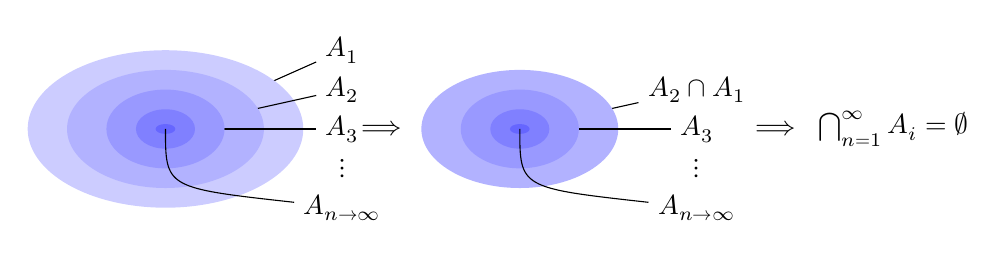
\begin{tikzpicture}[scale=0.5]
    \def\one{(4.5,2.5) ellipse (3.5 cm and 2 cm)};
    \def\two{(4.5,2.5) ellipse (2.5 cm and 1.5 cm)};
    \def\three{(4.5,2.5) ellipse (1.5 cm and 1 cm)};
    \def\four{(4.5,2.5) ellipse (0.75 cm and 0.5 cm)};
    \def\five{(4.5,2.5) ellipse (0.25 cm and 0.125 cm)};
    \node (n1) at (9,4.5) {$A_{1}$};
    \draw (4.5,2.5) -- (n1);
    \fill[fill=blue!20]\one;
    \node (n2) at (9,3.5) {$A_{2}$};
    \draw (4.5,2.5) -- (n2);
    \fill[fill=blue!30]\two;
    \node (n3) at (9,2.5) {$A_{3}$};
    \draw (4.5,2.5) -- (n3);
    \fill[fill=blue!40]\three;
    \fill[fill=blue!50]\four;
    \fill[fill=blue!60]\five;
    \node (n4) at (9,1.5) {$\vdots$};
    \node (nn) at (9,0.5) {$A_{n\to \infty}$};
    \draw (4.5,2.5) .. controls +(down:1.5cm) .. (nn);
    \node (meioum) at (10,2.5) {$\Longrightarrow$};
    \def\twoz{(13.5,2.5) ellipse (2.5 cm and 1.5 cm)};
    \def\threez{(13.5,2.5) ellipse (1.5 cm and 1 cm)};
    \def\fourz{(13.5,2.5) ellipse (0.75 cm and 0.5 cm)};
    \def\fivez{(13.5,2.5) ellipse (0.25 cm and 0.125 cm)};
    \node (n22) at (18,3.5) {$A_{2} \cap A_{1}$};
    \draw (13.5,2.5) -- (n22);
    \fill[fill=blue!30]\twoz;
    \node (n32) at (18,2.5) {$A_{3}$};
    \draw (13.5,2.5) -- (n32);
    \fill[fill=blue!40]\threez;
    \fill[fill=blue!50]\fourz;
    \fill[fill=blue!60]\fivez;
    \node (n42) at (18,1.5) {$\vdots$};
    \node (nn2) at (18,0.5) {$A_{n \to \infty}$};
    \draw (13.5,2.5) .. controls +(down:1.5cm) .. (nn2);
    \node (meiodois) at (20,2.5) {$\Longrightarrow$};
    \node (final) at (23,2.5) {$\bigcap_{n=1}^{\infty}A_{i} = \emptyset$};
\end{tikzpicture}
\end{center}

\begin{proposition}
\protect\hypertarget{prp:axiomas}{}\label{prp:axiomas}Dados os axiomas \(Ax_{1}(K),Ax_{2}(K),Ax_{3}(K)\), o axioma 4 é equivalente ao axioma \(Ax'_{3}(K)\), ou seja, uma probabilidade finitamente aditiva é uma medida de probabilidade se e somente se é contínua no vazio.
\end{proposition}

A prova de que a \(\sigma\)-aditividade implica o axioma 4 é consequência da prova da proposição anterior, dado que \(\bigcap_{n=1}^{\infty}A_{n} = \emptyset\). Para demonstrar o contrário (que \(Ax_{1}(K) + Ax_{2}(K) + Ax_{3}(K) + Ax_{4}(K) \rightarrow Ax'_{3}(K)\)), tomemos uma sequência infinita de eventos \(\{A_{i}\}_{i \ge 1}\) em \(\mathcal{A} : A_{i} \cap A_{j} = \emptyset \; \forall i \neq j\). Devemos ver que \(P(\bigcup_{n=1}^{\infty}) = \sum_{n=1}^{\infty}P(A_{n})\). Seja \(A = \bigcup_{n=1}^{\infty}A_{n} = (\bigcup_{n=1}^{k}A_{n}) \cup (\bigcup_{n=k+1}^{\infty}A_{n})\). Tem-se que:

\begin{equation*}
P(A) = P\left(\bigcup_{n=1}^{k}A_{n}\right) + P\left(\bigcup_{n=k+1}^{\infty}A_{n}\right) = \sum_{n=1}^{k}P(A_{n}) +P\left(\bigcup_{n=k+1}^{\infty}A_{n}\right)
\end{equation*}

Seja \(B_{k} = \bigcup_{n=k+1}^{\infty}A_{n}\). Note que \(B_{k} \downarrow \emptyset\) quando \(k \to \infty\) de modo que \(P(B_{k})\xrightarrow[k \to \infty]{}0\), logo:

\begin{equation*}
\lim_{k \to \infty}\sum_{n=1}^{k}P(A_{n}) = \sum_{n=1}^{\infty}P(A_{n})
\end{equation*}

\begin{corollary}
Os seguintes sistemas são equivalentes:

\begin{equation*}
Ax_{1}(K),Ax_{2}(K),Ax'_{3}(K) \equiv Ax_{1}(K),Ax_{2}(K),Ax_{3}(K),Ax_{4}(K)
\end{equation*}
\end{corollary}

\hypertarget{propriedades-de-probabilidade}{%
\subsection{Propriedades de probabilidade}\label{propriedades-de-probabilidade}}

Seja \(P\) uma probabilidade em uma \(\sigma\)-álgebra \(\mathcal{A}\). Suponhamos que todo \(A\) abaixo pertença à \(\mathcal{A}\). Então as seguintes propriedades são consequências dos axiomas:

\begin{itemize}
\tightlist
\item
  \textbf{P1}: \(P(A^{c}) = 1 - P(A)\);
\item
  \textbf{P2}: \(0 \le P(A) \le 1\);
\item
  \textbf{P3}: \(A_{1} \subset A_{2} \Rightarrow P(A_{1}) \le P(A_{2})\);
\item
  \textbf{P4}: \(P(\bigcup_{i=1}^{n}A_{i}) \le \sum_{i=1}^{n}P(A_{i})\);
\item
  \textbf{P5}: \(P(\bigcup_{i=1}^{\infty}A_{i}) \le \sum_{i=1}^{\infty}P(A_{i})\);
\end{itemize}

Com essas propriedades, podemos então definir um modelo probabilístico. Sejam:

\begin{itemize}
\tightlist
\item
  \textbf{a}) Um espaço amostral: \(\Omega \neq \emptyset\);
\item
  \textbf{b}) Uma \(\sigma\)-álgebra em \(\Omega\): \(\mathcal{A}\);
\item
  \textbf{c}) Uma medida de probabilidade em \(\mathcal{A}\): \(P\).
\end{itemize}

\begin{definition}
Um espaço de probabilidade é uma terna \((\Omega,\mathcal{A},P)\) seguindo \textbf{a},\textbf{b} e \textbf{c}.
\end{definition}

\hypertarget{probabilidade-condicional-e-independuxeancia}{%
\subsection{Probabilidade Condicional e Independência}\label{probabilidade-condicional-e-independuxeancia}}

Considere o seguinte experimento: um dado é lançado duas vezes e anota-se a dupla de resultados. Temos que:

\begin{equation*}
\Omega = \{(i,j) : 1 \le i \le 6; 1 \le j \le 6; i,j, \in \mathbb{Z}\}
\end{equation*}

Sejam os seguintes eventos:

\begin{itemize}
\tightlist
\item
  \(A = "\textit{em cada lançamento o valor observado é } \le 2"\);
\item
  \(B = "\textit{a soma dos resultados é igual a 4}"\).
\end{itemize}

\begin{align*}
A &= \{(1,1),(1,2),(2,1),(2,2)\} \\
B &= \{(1,3),(3,1),(2,2)\}
\end{align*}

Já que \(\#\Omega = |\Omega| = 36\), e pela equiprobabilidade dos eventos (considerando que os dados são honestos), temos que:

\begin{align*}
P(A) &= \frac{|A|}{|\Omega|} = \frac{4}{36} \\
P(B) &= \frac{|B|}{|\Omega|} = \frac{3}{36}
\end{align*}

Além disso, \((A \cap B) = \{(2,2)\}; P(A \cap B) = 1/36\). Suponha que \(A\) ocorre com \(P(A) > 0\), e que \(B\) é o evento de interesse. Assumindo a potencial ocorrência de \(A\), qual é a probabilidade de \(B\) ocorrer. Nesse caso \(P(B|A) = 1/4\).

\begin{definition}[Probabilidade condicional]
Sejam \(A\) e \(B\) eventos em \(\mathcal{A}\), com \(P(A) > 0\). A probabilidade condicional \(P(B|A)\) é definida como:

\begin{equation}
P(B|A) = \frac{P(A \cap B)}{P(A)}
\label{eq:probcond}
\end{equation}

ou equivalentemente:

\begin{equation}
P(A \cap B) = P(B|A)P(A)
\label{eq:probconddif}
\end{equation}
\end{definition}

\begin{example}

Considere uma urna com 5 bolas, sendo 3 vermelhas e 2 brancas. O experimento consiste de 2 retiradas sucessivas de uma bola da urna (sem reposição). Considere os eventos \(A_{1} = \textit{Cor da primeira bola}\) e \(A_{2} = \textit{Cor da segunda bola}\):

\begin{align*}
P(A_{1} = B) = \frac{2}{5} \;&,\; P(A_{1} = V) = \frac{3}{5} \\
P(A_{2} = B|A_{1} = B) = \frac{1}{4} \;&,\; P(A_{2} = V|A_{1} = B) = \frac{3}{4} \\
P(A_{2} = B|A_{1} = V) = \frac{2}{4} \;&,\; P(A_{2} = V|A_{1} = V) = \frac{2}{4}
\end{align*}

Podemos visualizar esse experimento com os seguintes diagrama e tabela de probabilidades:

\begin{center}
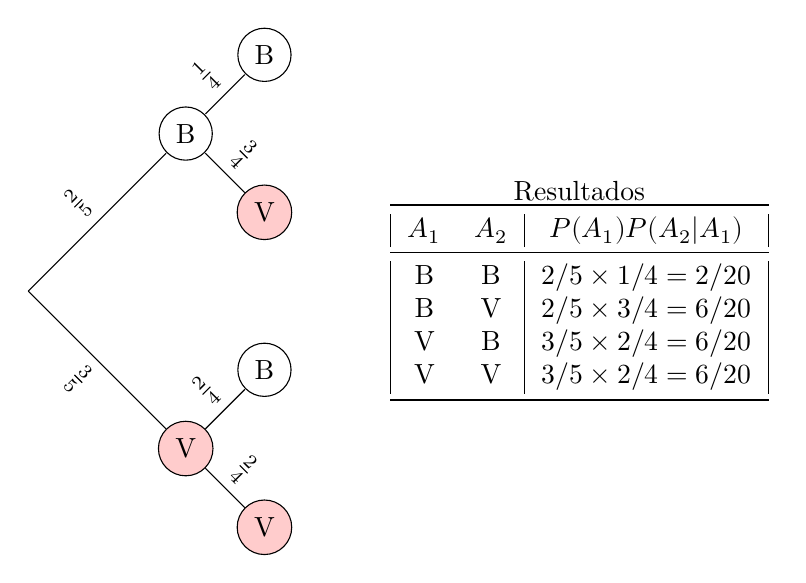
\begin{tikzpicture}
    \draw (0,0) -- (1.75,1.75) node[midway,sloped,above] {$\frac{2}{5}$};
    \draw (2,2) node[circle,draw] {B};
    \draw (2.25,2.25) -- (2.75,2.75) node[midway,sloped,above] {$\frac{1}{4}$};
    \draw (3,3) node[circle,draw] {B};
    \draw (2.25,1.75) -- (2.75,1.25) node[midway,sloped,above] {$\frac{3}{4}$};
    \draw (3,1) node[circle,draw,fill=red!20] {V};
    \draw (0,0) -- (1.75,-1.75) node[midway,sloped,below] {$\frac{3}{5}$};
    \draw (2,-2) node[circle,draw,fill=red!20] {V};
    \draw (2.25,-2.25) -- (2.75,-2.75) node[midway,sloped,above] {$\frac{2}{4}$};
    \draw (3,-1) node[circle,draw] {B};
    \draw (2.25,-1.75) -- (2.75,-1.25) node[midway,sloped,above] {$\frac{2}{4}$};
    \draw (3,-3) node[circle,draw,fill=red!20] {V};
    \node [shape=rectangle, align=center](table1) at (7,0) {
        Resultados \\
        \begin{tabular}{|cc|c|} \toprule
        $A_{1}$ & $A_{2}$  & $P(A_{1})P(A_{2}|A_{1})$ \\ \midrule
        B & B & $2/5 \times 1/4 = 2/20$ \\
        B & V & $2/5 \times 3/4 = 6/20$ \\
        V & B & $3/5 \times 2/4 = 6/20$ \\
        V & V & $3/5 \times 2/4 = 6/20$ \\ \bottomrule
        \end{tabular}
    };
\end{tikzpicture}
\end{center}

\end{example}

\begin{definition}[Eventos independentes]
\leavevmode

\begin{itemize}
\tightlist
\item
  \textbf{a}) Os eventos \(A\) e \(B\) são independentes (denotados como \(A \perp B\)) se \(P(A \cap B) = P(A)P(B)\);
\item
  \textbf{b}) \(\{A_{i}, i \in \mathbb{I}\}\) são independentes se \(P\left(\bigcap_{i \in \mathcal{J}}A_{i}\right) = \prod_{i \in \mathcal{J}}P(A_{i}), \; \forall\text{ subfamílias } \mathcal{J} \text{ de índices em } \mathbb{I}\).
\end{itemize}

\end{definition}

Disso segue que, sendo \(A\) e \(B\) dois eventos, as seguintes propriedades são válidas:

\begin{enumerate}
\def\labelenumi{\arabic{enumi}.}
\tightlist
\item
  Se \(P(A) = 0 \Rightarrow P(A \cap B) = 0 \; \forall B\), ou seja, \(A \perp B\);
\item
  Se \(P(B) = 1 \Rightarrow P(A \cap B) = 0 \; \forall A\), ou seja, \(A \perp B\);
\item
  \(A\) é independente dele mesmo se e somente se \(P(A) = 0\) ou \(P(A) = 1\);
\item
  \(A \perp B \Rightarrow A \perp B^{c}, A^{c} \perp B, A^{c} \perp B^{c}\);
\item
  As seguintes proposições são equivalentes:

  \begin{itemize}
  \item
    \begin{enumerate}
    \def\labelenumii{\alph{enumii})}
    \tightlist
    \item
      \((A \perp B) \Rightarrow P(B|A) = P(B)\) e \(P(B|A^{c}) = P(B)\);
    \end{enumerate}
  \item
    \begin{enumerate}
    \def\labelenumii{\alph{enumii})}
    \setcounter{enumii}{1}
    \tightlist
    \item
      \(P(B|A) = P(B) \Rightarrow A \perp B\);
    \end{enumerate}
  \item
    \begin{enumerate}
    \def\labelenumii{\alph{enumii})}
    \setcounter{enumii}{2}
    \tightlist
    \item
      \(P(B|A^{c}) = P(B) \Rightarrow A \perp B\).
    \end{enumerate}
  \end{itemize}
\end{enumerate}

\begin{theorem}[Teorema das Probabilidades Totais]
\leavevmode

\begin{enumerate}
\def\labelenumi{\arabic{enumi}.}
\tightlist
\item
  Dados \(A\) e \(B\) eventos em \(\mathcal{F}\):
\end{enumerate}

\begin{equation*}
P(A) = P(A|B)P(B) + P(A|B^{c})P(B^{c})
\end{equation*}

\begin{enumerate}
\def\labelenumi{\arabic{enumi}.}
\setcounter{enumi}{1}
\tightlist
\item
  No geral, se \(B_{1},B_{2}, \ldots, B_{n}\) é uma partição de \(\Omega\), então:
\end{enumerate}

\begin{equation}
P(A) = \sum_{i=1}^{n}P(A|B_{i})P(B_{i})
\label{eq:teorprobtotal}
\end{equation}

\end{theorem}

\textbf{Demonstração}: Note que \(A = (A \cap B) \cup (A \cap B^{c})\) e \((B \cap B^{c}) = \emptyset\) e \((B \cup B^{c}) = \Omega\). Além disso, \((A \cap B) \cap (A \cap B^{c}) = \emptyset\), logo \(P(A) = P(A \cap B) + P(A \cap B^{c})\). Como, por definição, \(P(A|B) = P(A \cap B) / P(B)\) e \(P(A|B^{c}) = P(A \cap B^{c}) / P(B^{c})\), temos que:

\begin{equation*}
P(A) = P(A|B)P(B) + P(A|B^{c})P(B^{c})
\end{equation*}

Para o caso geral, temos que \(\{B_{i}\}_{i=1}^{n} , \; (B_{i} \cap B_{j}) = \emptyset \; \forall i,j\) e \(\bigcup_{i=1}^{n}B_{i} = \Omega\). Logo:

\begin{align*}
A &= (A \cap B_{1}) \cup (A \cap B_{2}) \cup \ldots \cup (A \cap B_{n}) \\
&\Downarrow \; \text{Pela }\sigma\text{-aditividade} \\
P(A) &= \sum_{i=1}^{n}P(A \cap B_{i})
\end{align*}

E como \(P(A|B_{i}) = P(A \cap B_{i}) \ P(B_{i})\):

\begin{equation*}
P(A) = \sum_{i=1}^{n}P(A|B_{i})P(B_{i})
\end{equation*}

\hypertarget{fuxf3rmula-de-poincaruxe9-e-teorema-de-bayes}{%
\subsection{Fórmula de Poincaré e Teorema de Bayes}\label{fuxf3rmula-de-poincaruxe9-e-teorema-de-bayes}}

\begin{theorem}[Fórmula de Poincaré]
Seja \(\{A_{i}\}_{i \ge 1} \subseteq \mathcal{F}\). Então:

\begin{equation}
\begin{split}
P\left(\bigcup_{i=1}^{n} A_{n}\right) = &\sum_{i=1}^{n}P(A_{i}) - \sum_{1 \le i_{1} < i_{2} \le n} P(A_{i_{1}} \cap A_{i_{2}}) + \sum_{1 \le i_{1} < i_{2} < i_{3} \le n} P(A_{i_{1}} \cap A_{i_{2}} \cap A_{i_{3}}) - \dots \\
&+ (-1)^{n+1} P(A_{1} \cap A_{2} \cap \ldots \cap A_{n})
\label{eq:formulapoincare}
\end{split}
\end{equation}
\end{theorem}

A demonstração da fórmula \eqref{eq:formulapoincare} é dada no exercício \ref{exr:exbj13}.

\begin{theorem}[Teorema de Bayes]
Seja \(\{B_{i}\}_{i=1}^{n}\) uma partição de \(\Omega\) e \(A\) um evento em \(\mathcal{F}\), temos que:

\begin{equation}
P(B_{i}|A) = \frac{P(A|B_{i})P(B_{i})}{\sum_{j=1}^{n}P(A|B_{j})P(B_{j})}
\label{eq:teoremabayes}
\end{equation}
\end{theorem}

O denominador de \eqref{eq:teoremabayes} é derivado do teorema das probabilidades totais, visto que \(\{B_{i}\}_{i=1}^{n}\) é uma partição de \(\Omega\).

\begin{lemma}
Sejam \(A_{1},A_{2}, \ldots, A_{n}\) eventos em \(\mathcal{F}\), logo:

\begin{equation*}
P\left(\bigcap_{i=1}^{n}A_{i}\right) = P(A_{1})P(A_{2}|A_{1})P(A_{3}|A_{1} \cap A_{2}) \ldots P(A_{n}|A_{1} \cap A_{2} \cap \ldots \cap A_{n-1})
\end{equation*}
\end{lemma}

\begin{proof}
Suponha a validade do lema anterior. Logo, seja \(D = (\bigcap_{i=1}^{n}A_{i})\):

\begin{align*}
P(A_{1} \cap \ldots \cap A_{n} \cap A_{n+1}) &= P(D \cap A_{n+1}) \\
&= P(D)P(A_{n+1}|D) \\
&= P(A_{1})P(A_{2}|A_{1}) \ldots P(A_{n}|A_{1} \cap \ldots \cap A_{n-1})P(A_{n+1}|A_{1} \cap \ldots \cap A_{n})
\end{align*}
\end{proof}

\newpage

\hypertarget{exercuxedcios}{%
\subsection{Exercícios}\label{exercuxedcios}}

\begin{exercise}[BJ1]

Sejam \(A, B\) e \(C\) eventos aleatórios. Identifique as seguintes equações e frases, casando cada equação expressa na notação de conjuntos com a correspondente frase na linguagem de eventos:

\begin{center}
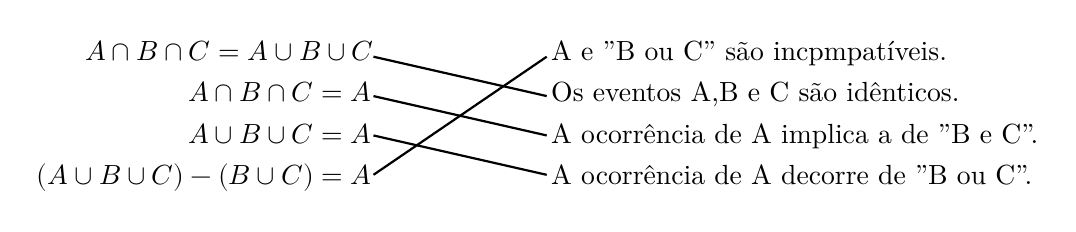
\begin{tikzpicture}
    \node (a) at (0,0) {$
        \begin{aligned}
            A \cap B \cap C = A \cup B \cup C &\\
            A \cap B \cap C = A &\\
            A \cup B \cup C = A &\\
            (A \cup B \cup C) - (B \cup C) = A &
        \end{aligned}$};
    \node (i) at (7.5,0) {$
        \begin{aligned}
            & \text{A e "B ou C" são incpmpatíveis.}\\
            & \text{Os eventos A,B e C são idênticos.}\\
            & \text{A ocorrência de A implica a de "B e C".}\\
            & \text{A ocorrência de A decorre de "B ou C".}
        \end{aligned}
    $};
    \draw[thick] (2.15,0.75) -- (4.35,0.25);
    \draw[thick] (2.15,0.25) -- (4.35,-0.25);
    \draw[thick] (2.15,-0.25) -- (4.35,-0.75);
    \draw[thick] (2.15,-0.75) -- (4.35,0.75);
\end{tikzpicture}
\end{center}

\end{exercise}

\begin{exercise}[BJ2]
\protect\hypertarget{exr:exbj2}{}\label{exr:exbj2}

A partir dos axiomas, prove a propriedade \(P5\):

\[
P\left(\bigcup_{n=i}^{\infty}A_{n}\right) \le \sum_{n=1}^{\infty}P(A_{n})
\]

\begin{proof}
Consideremos uma prova por indução para \(n \to \infty\):

Para \(n=2\):

\[
P(A_{1} \cup A_{2}) = P(A_{1}) + P(A_{1}^{c} \cap A_{2})
\]

Considerando que \((A_1^{c} \cap A_{2}) \subset A_{2}\) e o fato de que \((A_{1}) \cap (A_{1}^{c} \cap A_{2}) = \emptyset\), temos pela propriedade \(P3\) que \(P(A_1^{c} \cap A_{2}) \le P(A_{2})\), de modo que:

\begin{align*}
P(A_{1} \cup A_{2}) &= P(A_{1}) + P(A_{1}^{c} \cap A_{2}) \le P(A_{2}) \\
&\le P(A_{1}) + P(A_{2})\\
&\le \sum_{i=1}^{2}P(A_{i})
\end{align*}

De modo semelhante, podemos fazer para \(n\):

\begin{align*}
P\left(\bigcup_{i=i}^{n}A_{i}\right) &= P(A_{1}) + P(A_{1}^{c} \cap A_{2}) + \dots \\
&\le P(A_{1}) + P(A_{2}) + \dots\\
&\le \sum_{i=1}^{n}P(A_{i})
\end{align*}

Consideremos então uma sequência de eventos \(A_{i}^{*},\forall i \in \{n+1,n+2,\dots\}\), disjuntos de \(A_{i}\). Denotemos ainda \(A = \left(\bigcup_{i = 1}^{n}A_{i}\right) \cup \left(\bigcup_{i=n+1}^{\infty}A_{i}\right)\). Pela aditividade infinita (ou ainda pela \(\sigma\)-aditividade), temos que:

\[
P\left(\bigcup_{n=i}^{\infty}A_{n}\right) \le \sum_{i=1}^{n}P(A_{i}) + P\left(\bigcup_{i=n+1}^{\infty}A_{i}\right)
\]

Que por serem disjuntos, pelo axioma \(Ax_{4}\) tem que \(\left(\bigcup_{i=n+1}^{\infty}A_{i}\right)\downarrow \emptyset\), de modo que \(P\left(\bigcup_{i=n+1}^{\infty}A_{i}\right) \to 0\). Logo, tem-se que:

\[
P\left(\bigcup_{n=i}^{\infty}A_{n}\right) \le \sum_{n=1}^{\infty}P(A_{n})
\]
\end{proof}

\end{exercise}

\begin{exercise}[BJ3]
\protect\hypertarget{exr:exbj3}{}\label{exr:exbj3}

Sejam \(A_{1}, A_{2},\dots\) eventos aleatórios. Mostre que:

\begin{enumerate}
\def\labelenumi{\alph{enumi})}
\tightlist
\item
  \(P\left(\bigcap_{k=1}^{n}A_{k}\right) \ge 1 - \sum_{k=1}^{n}P(A_{k}^{c})\)
\end{enumerate}

\begin{proof}
Por De Morgan temos que \(\bigcap_{k=1}^{n}A_{k} = \left(\bigcup_{k=1}^{n}A_{k}^{c}\right)^{c}\), de modo que:

\begin{align*}
P\left(\bigcap_{k=1}^{n}A_{k}\right) &= P\left(\bigcup_{k=1}^{n}A_{k}^{c}\right)^{c} \\
&= 1 - P\left(\bigcup_{k=1}^{n}A_{k}^{c}\right) \xRightarrow[]{\text{Por P4}} P\left(\bigcup_{k=1}^{n}A_{k}^{c}\right) \le \sum_{k=1}^{n}P\left(A_{k}^{c}\right) \\
&\ge 1 - \sum_{k=1}^{n}P\left(A_{k}^{c}\right)
\end{align*}
\end{proof}

\begin{enumerate}
\def\labelenumi{\alph{enumi})}
\setcounter{enumi}{1}
\tightlist
\item
  Se \(P(A_{k}) \ge 1 - \epsilon\) para \(k = 1,2,\dots,n\), então \(P(\bigcap_{k=1}^{n}A_{k}) \ge 1 - n\epsilon\)
\end{enumerate}

\begin{proof}
É fácil ver que:

\[
P(A_{k}) \ge 1 - \epsilon \Rightarrow P(A_{k}^{c}) \le 1 - (1-\epsilon) = \epsilon
\]

E de modo semelhante ao que foi feito na questão anterior (utilizando De Morgan), temos que:

\begin{align*}
P\left(\bigcap_{k=1}^{n}A_{k}\right) = P\left(\bigcup_{k=1}^{n}A_{k}^{c}\right)^{c} &= 1 - P\left(\bigcup_{k=1}^{n}A_{k}^{c}\right)\\
&\ge 1 - \sum_{k=1}^{n}P\left(A_{k}^{c}\right) \\
&\ge 1 - \sum_{k=1}^{n}\epsilon\\
&\ge 1 - n\epsilon
\end{align*}
\end{proof}

\begin{enumerate}
\def\labelenumi{\alph{enumi})}
\setcounter{enumi}{2}
\tightlist
\item
  \(P\left(\bigcap_{k=1}^{\infty}A_{k}\right) \ge 1 - \sum_{k=1}^{\infty}P(A_{k}^{c})\)
\end{enumerate}

\begin{proof}
De maneira semelhante ao que foi visto na prova da letra \textbf{a}, temos que:

\begin{align*}
P\left(\bigcap_{k=1}^{\infty}A_{k}\right) &= P\left(\bigcup_{k=1}^{\infty}A_{k}^{c}\right)^{c} \\
&= 1 - P\left(\bigcup_{k=1}^{\infty}A_{k}^{c}\right) \xRightarrow[]{\text{Por P5}} P\left(\bigcup_{k=1}^{n}A_{k}^{c}\right) \le \sum_{k=1}^{\infty}P\left(A_{k}^{c}\right) \\
&\ge 1 - \sum_{k=1}^{\infty}P\left(A_{k}^{c}\right)
\end{align*}

Para ver a demonstração da propriedade \(P5\), vide exercício \ref{exr:exbj2}.
\end{proof}

\end{exercise}

\begin{exercise}[BJ4]

Demonstre as seguintes propriedades:

\begin{enumerate}
\def\labelenumi{\alph{enumi})}
\tightlist
\item
  Se \(P(A_{n}) = 0\) para \(n = 1,2,\dots\), então \(P\left(\bigcup_{n=1}^{\infty}A_{n}\right) = 0\).
\end{enumerate}

\begin{proof}
Utilizando a propriedade \(P5\), temos que:

\begin{align*}
P\left(\bigcup_{n=1}^{\infty} A_{n}\right) &\le \sum_{n=1}^{\infty}P(A_{n}) \\
&\le \sum_{n=1}^{\infty}0 \\
&\le 0 \\
&\;\Big\downarrow \;\text{Por } P2\\
P\left(\bigcup_{n=1}^{\infty} A_{n}\right) &= 0
\end{align*}
\end{proof}

\begin{enumerate}
\def\labelenumi{\alph{enumi})}
\setcounter{enumi}{1}
\tightlist
\item
  Se \(P(A_{n}) = 1\) para \(n = 1,2,\dots\), então \(P\left(\bigcap_{n=1}^{\infty}A_{n}\right) = 1\).
\end{enumerate}

\begin{proof}
Levando em consideração que se \(P(A_{n}) = 1 \Rightarrow P(A_{n}^{c}) = 0\) (pela propriedade \(P1\)), utilizando De Morgan e a prova da letra \textbf{c} do exercício \ref{exr:exbj3}, temos que:

\begin{align*}
P\left(\bigcap_{n=1}^{\infty}A_{n}\right) &\ge 1 - \sum_{n=1}^{\infty} P(A_{n}^{c}) \\
&\ge 1 - \sum_{n=1}^{\infty}0 \\
&\ge 1 - 0 \\
&\ge 1 \\
&\;\Big\downarrow \;\text{Por } P2\\
P\left(\bigcap_{n=1}^{\infty}A_{n}\right) &= 1
\end{align*}
\end{proof}

\end{exercise}

\begin{exercise}[BJ6]

Seja \(\Omega\) um conjunto não-vazio.

\begin{enumerate}
\def\labelenumi{\alph{enumi})}
\tightlist
\item
  Prove: se \(\mathcal{A}\) e \(\mathcal{B}\) são \(\sigma\)-álgebras de subconjuntos de \(\Omega\), então \((\mathcal{A} \cap \mathcal{B})\) também é uma \(\sigma\)-álgebra.
\end{enumerate}

\begin{proof}
Para que \(\mathcal{A} \cap \mathcal{B}\) seja uma \(\sigma\)-álgebra, é necessário que cumpram-se os axiomas \(Ax_{1}, Ax_{2}\) e \(Ax_{3}\):

\begin{itemize}
\tightlist
\item
  \(Ax_{1}\): Sabemos que \(\Omega \in \mathcal{A}\) e \(\Omega \in \mathcal{B}\), logo sabemos que \(\Omega \in (\mathcal{A} \cap \mathcal{B})\);
\item
  \(Ax_{2}\): Seja um evento \(E \in (\mathcal{A} \cap \mathcal{B})\), sabemos então que \(E \in \mathcal{A}\) e \(E \in \mathcal{B}\), logo \(E^{c} \in \mathcal{A}\) e \(E^{c} \in \mathcal{B}\), portanto \(E^{c} \in (\mathcal{A} \cap \mathcal{B})\);
\item
  \(Ax_{3}\): Sejam dois eventos, \(E_{1} \in (\mathcal{A} \cap \mathcal{B})\) e \(E_{2} \in (\mathcal{A} \cap \mathcal{B})\). Com isso, temos que \(E_{1}, E_{2} \in \mathcal{A}\) e \(E_{1}, E_{2} \in \mathcal{B}\), portanto \((E_{1} \cup E_{2}) \in \mathcal{A}\) e \(E_{1} \cup E_{2} \in \mathcal{B}\), logo \((E_{1} \cup E_{2}) \in (\mathcal{A} \cap \mathcal{B})\).
\end{itemize}

Como os três axiomas foram cumpridos, temos que \((\mathcal{A} \cap \mathcal{B})\) é uma \(\sigma\)-álgebra.
\end{proof}

\begin{enumerate}
\def\labelenumi{\alph{enumi})}
\setcounter{enumi}{1}
\tightlist
\item
  Generalize o item (a): se \(\mathcal{A}_{i}, i \in \mathcal{I}\), são \(\sigma\)-álgebras de partes de \(\Omega\), onde \(\mathcal{I}\) é um conjunto não-vazio de índices, então \(\bigcap_{i \in \mathcal{I}}\mathcal{A}_{i}\) também é uma \(\sigma\)-álgebra.
\end{enumerate}

\begin{proof}
Como anteriormente, temos que mostrar que \(\bigcap_{i \in \mathcal{I}}\mathcal{A}_{i}\) cumpre os axiomas \(Ax_{1}, Ax_{2}\) e \(Ax_{3}\):

\begin{itemize}
\tightlist
\item
  \(Ax_{1}\): Sabemos que \(\Omega \in \mathcal{A}_{i}, \; \forall i \in \mathcal{I}\), logo sabemos que \(\Omega \in \bigcap_{i \in \mathcal{I}}\mathcal{A}_{i}\);
\item
  \(Ax_{2}\): Seja um evento \(E \in \bigcap_{i \in \mathcal{I}}\mathcal{A}_{i}\), sabemos então que \(E \in \mathcal{A}_{i}, \; \forall i \in \mathcal{I}\), logo \(E^{c} \in \mathcal{A}_{i}, \; \forall i \in \mathcal{A}\), portanto \(E^{c} \in \bigcap_{i \in \mathcal{I}}\mathcal{A}_{i}\);
\item
  \(Ax_{3}\): Sejam dois eventos, \(E_{1} \in \bigcap_{i \in \mathcal{I}}\mathcal{A}_{i}\) e \(E_{2} \in \bigcap_{i \in \mathcal{I}}\mathcal{A}_{i}\). Com isso, temos que \(E_{1}, E_{2} \in \mathcal{A}_{i}, \; \forall i \in \mathcal{I}\), portanto \((E_{1} \cup E_{2}) \in \mathcal{A}_{i}, \; \forall i \in \mathcal{I}\), logo \((E_{1} \cup E_{2}) \in \bigcap_{i \in \mathcal{I}}\mathcal{A}_{i}\).
\end{itemize}

Vemos portanto que, por cumprir os axiomas \(Ax_{1}, Ax_{2}\) e \(Ax_{3}\), \(\bigcap_{i \in \mathcal{I}}\mathcal{A}_{i}\) é também uma \(\sigma\)-álgebra.
\end{proof}

\begin{enumerate}
\def\labelenumi{\alph{enumi})}
\setcounter{enumi}{2}
\tightlist
\item
  Seja \(\mathbb{C}\) uma classe de subconjuntos de \(\Omega\). Mostre que existe \emph{pelo menos uma} \(\sigma\)-álgebra que contém \(\mathbb{C}\).
\end{enumerate}

\begin{proof}
É fácil ver que a maior classe de subconjuntos de \(\Omega\) é o conjunto das partes de \(\Omega\), denotado como \(\mathcal{P}(\Omega)\) (definido no exemplo \ref{exm:powerset}). Assim, temos que \(\mathbb{C} \subseteq \mathcal{P}(\Omega)\), de modo que, pelo menos a \(\sigma\)-álgebra formada por \(\mathcal{P}(\Omega)\) contém \(\mathbb{C}\).
\end{proof}

\begin{enumerate}
\def\labelenumi{\alph{enumi})}
\setcounter{enumi}{3}
\tightlist
\item
  Visando a plena utilização dos itens (b) e (c), como você definiria ``a menor \(\sigma\)-álgebra contendo \(\mathbb{C}\)'', onde \(\mathcal{C}\) é uma classe de subconjuntos de \(\Omega\)?
\end{enumerate}

\begin{proof}
Considere que temos \(\sigma\)-álgebras de partes de \(\Omega\), \(\mathcal{A}_{i}\) com \(i \in \mathbb{I}\) (sendo \(\mathbb{I}\) um conjunto não-vazio de índices), tais que \(\mathbb{C} \in \mathcal{A}_{i}: \; \forall i \in \mathbb{I}\). Assim, sabemos que algum dos \(\mathcal{A}_{i}\) é a menor \(\sigma\)-álgebra que contém \(\mathbb{C}\), de modo que \(\bigcap_{i \in \mathbb{I}}A_{i}\) será a menor \(\sigma\)-álgebra que contém \(\mathbb{C}\).
\end{proof}

\end{exercise}

\begin{exercise}[BJ9]

Uma caixa contém \(2n\) sorvetes, \(n\) do sabor \(A\) e \(n\) do sabor \(B\). De um grupo de \(2n\) pessoas, \(a < n\) preferem o sabor \(A\), \(b < n\) o sabor \(B\) e \(2n-(a+b)\) não tem preferência. Demonstre: se os sorvetes são distribuídos ao acaso, a probabilidade de que a preferência de todas as pessoas seja respeitada é de \(\binom{2n-a-b}{n-a}/\binom{2n}{n}\).

\begin{proof}
Sabendo que a ordem de entrega dos \(n\) sorvetes de cada sabor, para as \(2n\) pessoas não importa, temos que a quantidade possível de entregas diferentes é:

\begin{equation*}
|\Omega| = \binom{2n}{n}
\end{equation*}

Considere que o evento \(R\) indica o caso em que todos tiveram sua preferência respeitada. Podemos ver que:

\begin{equation*}
P(R) = \frac{|R|}{|\Omega|} = \frac{|R|}{\binom{2n}{n}}
\end{equation*}

Para que \(R\) ocorra, é necessário que as \(a\) pessoas que preferem \(A\) recebam esse sabor, bem como as \(b\) pessoas que preferem \(B\). Dessa forma, temos que distribuir os \(2n-(a+b)\) sorvetes restantes para as pessoas que não tem preferência. Assim, primeiramente temos os \(n-a\) sorvetes do sabor \(A\) que não foram alocados, de forma que:

\begin{equation}
\binom{2n-a-b}{n-a} = \frac{(2n-a-b)!}{(2n-a-b-n+a)!(n-a)!} = \frac{(2n-a-b)!}{(n-b)!(n-a)!}\\
\label{eq:aloca}
\end{equation}

E podemos mostrar que, caso fossemos alocar os \(n-b\) sorvetes do sabor \(B\) para as \(2n-(a+b)\) pessoas sem preferência, teríamos:

\begin{equation}
\binom{2n-a-b}{n-b} = \frac{(2n-a-b)!}{(2n-a-b-n+b)!(n-b)!} = \frac{(2n-a-b)!}{(n-a)!(n-b)!}\\
\label{eq:alocb}
\end{equation}

Como \eqref{eq:aloca} e \eqref{eq:aloca} são iguais, podemos ver que a alocação dos sorvetes restantes não depende de qual sabor já foi alocado. Assim, temos que \(|R| = \binom{2n-a-b}{n-a} = \binom{2n-a-b}{n-b}\), portanto:

\begin{equation*}
P(R) = \frac{|R|}{|\Omega|} = \frac{\binom{2n-a-b}{n-a}}{\binom{2n}{n}}
\end{equation*}
\end{proof}

\end{exercise}

\begin{exercise}[BJ10]

Suponhamos que dez cartas estejam numeradas de 1 até 10. Das dez cartas, retira-se uma de cada vez, ao acaso e sem reposição, até retirar-se o primeiro número par. Conta-se o número de retiradas necessárias. Exiba um bom modelo probabilístico para esse experimento.

\begin{proof}
Dada essa formulação, temos que 5 cartas são pares e 5 são ímpares. Assim, considere o evento \(\{Y_{k} \;: 1 \le k \le 6 ; k \in \mathbb{Z}\}\) em que \(k\) indica que a \(k\)-ésima retirada contém a primeira carta par. Assim, por exemplo, \(Y_{1}\) indica o evento em que a primeira carta retirada é par, \(Y_{2}\) o evento em que a segunda carta retirada é par, e assim por diante.

O nosso espaço amostral é (visto que o número da carta não importa, apenas se é \(P = "\text{par}"\) ou \(I = "\text{ímpar}"\)):

\begin{equation*}
\Omega = \{(P), (I,P), (I,I,P), (I,I,I,P), (I,I,I,I,P), (I,I,I,I,I,P)\}\\
\end{equation*}

É fácil ver que não é possível ter \(\{Y_{k} : k \ge 7\}\), já que as cartas são retiradas sem reposição. Podemos facilmente calcular as probabilidades de cada evento em \(\Omega\), como segue:

\begin{align*}
P(Y_{1}) &= \frac{5}{10} = \frac{1}{2}\\
P(Y_{2}) &= \frac{5}{10} \cdot \frac{5}{9}  = \frac{5}{18}\\
P(Y_{3}) &= \frac{5}{10} \cdot \frac{4}{9} \cdot \frac{5}{8} = \frac{5}{36}\\
P(Y_{4}) &= \frac{5}{10} \cdot \frac{4}{9} \cdot \frac{3}{8} \cdot \frac{5}{7} = \frac{5}{84}\\
P(Y_{5}) &= \frac{5}{10} \cdot \frac{4}{9} \cdot \frac{3}{8} \cdot \frac{2}{7} \cdot \frac{5}{6} = \frac{5}{252}\\
P(Y_{6}) &= \frac{5}{10} \cdot \frac{4}{9} \cdot \frac{3}{8} \cdot \frac{2}{7} \cdot \frac{1}{6} \cdot \frac{5}{5} = \frac{1}{252}\\
\end{align*}

Podemos ver que \(\sum_{k = 1}^{6}P(Y_{k}) = 1\), e além disso, podemos denotar as probabilidades a partir da seguinte função:

\begin{equation}
P(Y_{k}) = \frac{5}{11-k} \cdot \prod_{n=1}^{k-1} \frac{6-n}{11-n}
\label{eq:bj10}
\end{equation}

A segunda parcela da equação \eqref{eq:bj10} é válida para \(k \ge 2\), pois ela representa as \(k-1\) cartas ímpares retiradas antes da primeira carta par, caso que só ocorre caso \(k \ge 2\).
\end{proof}

\end{exercise}

\begin{exercise}[BJ11]

Para cada um dos seguintes experimentos, descreva um espaço de probabilidade que sirva de modelo:

\begin{enumerate}
\def\labelenumi{\alph{enumi})}
\tightlist
\item
  Seleciona-se um ponto, ao acaso, do quadrado unitário
\end{enumerate}

\begin{equation*}
\{(x,y) : 0 \le x \le 1, 0 \le y \le 1\}
\end{equation*}

\begin{proof}
Temos que:

\begin{equation*}
\Omega = \{(x,y) \in [0,1] \times [0,1] \subset \mathbb{R}^{2}\}
\end{equation*}

Pela continuidade no vazio, é necessário que a probabilidade de ocorrência de um determinado ponto ser igual a zero, de modo que uma medida de probabilidade possível é por meio de intervalos. Considerando que \(x \sim U(0,1)\) e \(y \sim U(0,1)\) (ou seja, \(x\) e \(y\) são uniformemente distribuídos), podemos encontrar a probabilidade de \((x,y) \in \mathbb{I}\), com \(\mathbb{I}\) sendo um intervalo no cartesiano \([0,1] \times [0,1] \in \mathbb{R}^{2}\), por meio da distribuição de probabilidade conjunta de \(x\) e \(y\).
\end{proof}

\begin{enumerate}
\def\labelenumi{\alph{enumi})}
\setcounter{enumi}{1}
\tightlist
\item
  Retiram-se cartas sucessivamente de um baralho de 52 cartas, ao acaso e \emph{com} reposição, até retirar-se o primeiro rei. Registra-se o número total de retiradas.
\end{enumerate}

\begin{proof}
Considere que \(\{Y: Y \in \{1,2,\dots\}\}\) indica a quantidade de retiradas necessárias até o primeiro rei. O espaço amostral é dado diretamente: \(\Omega = \{1,2,3,\dots\}\). Temos que, para cada retirada, a probabilidade da carta ser um rei é \(4/52 = 1/13\) (considerando que temos 4 reis no baralho), e a probabilidade de não ser é de \(48/52 = 12/13\). Assim, a probabilidade de que a primeira retirada seja um rei é de:

\begin{equation*}
P(Y = 1) = \frac{1}{13}
\end{equation*}

Caso isso não ocorra, a probabilidade de que o primeiro rei ocorra na segunda retirada é de:

\begin{equation*}
P(Y = 2) = \frac{12}{13} \cdot \frac{1}{13}
\end{equation*}

É possível verificar que, para todo \(n \in \mathcal{N}\) a probabilidade de que o primeiro rei ocorra na retirada \(n\) é de:

\begin{equation*}
P(Y = n) = \left(\frac{12}{13}\right)^{n-1} \cdot \left(\frac{1}{13}\right)
\end{equation*}

Esse modelo de probabilidade é denotado modelo geométrico.
\end{proof}

\begin{enumerate}
\def\labelenumi{\alph{enumi})}
\setcounter{enumi}{2}
\tightlist
\item
  Quinze bolas são retiradas, ao acaso e \emph{com} reposição, de uma urna contendo 5 bolas vermelhas, 9 bolas pretas e uma bola branca. Observa-se o número que ocorre cada cor.
\end{enumerate}

\begin{proof}
Sejam os eventos \(V, P \text{ e } B\) o número de vezes que as retiradas foram de bolas vermelhas, pretas e brancas, respectivamente. É necessário (pela definição do modelo) que \(V + P + B = 15\), mas consideremos o caso em que o número de retiradas seja \(n\). Assim, para \(n = 1\), o espaço amostral \(\Omega\) é:

\begin{equation*}
\Omega = \{(V),(P),(B)\}
\end{equation*}

E as probabilidades de cada evento são:

\begin{align*}
P(V = 1) &= \frac{5}{15} \\
P(P = 1) &= \frac{9}{15} \\
P(B = 1) &= \frac{1}{15}
\end{align*}

Para \(n=2\) bolas retiradas, temos que o espaço amostral é:

\begin{align*}
\Omega = \{&(V,V), (V,P), (V,B), \\
&(P,V), (P,P), (P,B), \\
&(B,V), (B,P), (B,B)\}
\end{align*}

E as probabilidades de cada evento são:

\begin{align*}
P(V,V) &= \frac{5}{15} \cdot \frac{5}{15}; P(V,P) = \frac{5}{15} \cdot \frac{9}{15}; P(V,B) = \frac{5}{15} \cdot \frac{1}{15};\\
P(P,V) &= \frac{9}{15} \cdot \frac{5}{15}; P(P,P) = \frac{9}{15} \cdot \frac{9}{15}; P(P,B) = \frac{9}{15} \cdot \frac{1}{15};\\
P(B,V) &= \frac{1}{15} \cdot \frac{5}{15}; P(B,P) = \frac{1}{15} \cdot \frac{9}{15}; P(B,B) = \frac{1}{15} \cdot \frac{1}{15}
\end{align*}

Aqui é possível ver o padrão que surge para esse problema. Temos que os eventos \(V,P,B\) formam uma permutação (com repetição) da quantidade de bolas retiradas. A fórmula para a permutação com repetição de \(n\) elementos, em que cada um aparece \(k_{1},k_{2}, \dots k_{j}\) vezes é dada por:

\begin{equation*}
P_{n}^{k_{1},k_{2},\dots,k_{j}} = \frac{n!}{k_{1}! \cdot k_{2}! \cdot \dots \cdot k_{j}!}
\end{equation*}

Assim, podemos considerar que cada evento irá aparecer uma quantidade \(V = v, P = p, B = b\) de vezes, com a seguinte probabilidade:

\begin{equation*}
P(V=v, P=p, B=b) = \frac{15!}{v!p!b!} \cdot \left(\frac{5}{15}\right)^{v} \cdot \left(\frac{9}{15}\right)^{p} \cdot \left(\frac{1}{15}\right)^{b} \; ; \text{com }v+p+b = 15
\end{equation*}

Caso seja necessário, podemos ainda generalizar para uma quantidade \(n : 1 \le n \le 15\) de retiradas:

\begin{equation*}
P(V=v, P=p, B=b) = \frac{n!}{v!p!b!} \cdot \left(\frac{5}{15}\right)^{v} \cdot \left(\frac{9}{15}\right)^{p} \cdot \left(\frac{1}{15}\right)^{b} \; ; \text{com }v+p+b = n
\end{equation*}

Em que verifica-se facilmente que é válido para os casos em que \(n=1\) e \(n=2\) demonstrados anteriormente.
\end{proof}

\begin{enumerate}
\def\labelenumi{\alph{enumi})}
\setcounter{enumi}{3}
\tightlist
\item
  O experimento (\textbf{c}) é realizado \emph{sem} reposição.
\end{enumerate}

\begin{proof}
Como temos 15 bolas que serão retiradas \emph{sem} reposição, o único evento possível após as 15 serem retiradas é:

\begin{equation*}
\Omega = \{(V=5,P=9,B=1)\}
\end{equation*}

E a probabilidade de isso ocorrer é 1 (visto que é o único evento no espaço amostral). Caso consideremos uma quantidade de retiradas \(n < 15\), temos que o modelo de probabilidade é diferente. Consideremos que \(V + P + B = n\) e que a quantidade de vezes que cada cor aparece é \(v,p\) e \(b\), respectivamente. Então, como a ordem com que as cores são retiradas não importa, a probabilidade de aparecer uma quantidade de bolas de cada cor é dada por:

\begin{equation*}
P(V=v,P=p,B=b) = \frac{\binom{5}{v}\binom{9}{p}\binom{1}{b}}{\binom{15}{n}}, \;\; v+p+b = n
\end{equation*}

Esse modelo de probabilidade é chamado de multinomial hipergeométrico, e é uma generalização do modelo hipergeométrico para mais de duas classes (como é o caso).
\end{proof}

\end{exercise}

\begin{exercise}[BJ12]

Retiram-se 4 cartas, ao acaso, de um baralho de 52 cartas. Registra-se o número de reis na amostra. Exiba um bom modelo probabilístico para este experimento se:

\begin{enumerate}
\def\labelenumi{\alph{enumi})}
\tightlist
\item
  As retiradas são feitas \emph{sem} reposição.
\end{enumerate}

\begin{proof}
Considerando que em um baralho usual tem 52 cartas, e que a ordem com que cada uma das 4 cartas retiradas da amostra não importa (apenas importa a quantidade de reis na amostra), a quantidade total de amostras possíveis é \(\binom{52}{4}\).

Como temos 4 reis no baralho, isso implica que há 48 cartas que são ``não-reis''. Dessa forma, se na amostra forem coletados \(k\) reis, serão coletados também \(4-k\) ``não-reis'', com os \(k\) reis podendo aparecer de \(\binom{4}{k}\) maneiras diferentes (não importa qual o rei foi registrado) e os \(4-k\) ``não-reis'' podem aparecer de \(\binom{48}{4-k}\) maneiras diferentes.

Assim, seja \(K\) o evento registrar \(k\) reis na amostra, a probabilidade \(P(K=k)\) é dada por:

\begin{equation}
P(K=k) = \frac{\binom{4}{k}\binom{48}{4-k}}{\binom{52}{4}}
\label{eq:hgeomex}
\end{equation}

Esse modelo é chamado de hipergeométrico, que vale quando sabemos a quantidades de sucessos totais na população, e queremos contar a quantidade de sucessos coletados em uma amostra finita da população (que também deve ser finita).
\end{proof}

\begin{enumerate}
\def\labelenumi{\alph{enumi})}
\setcounter{enumi}{1}
\tightlist
\item
  As retiradas são feitas \emph{com} reposição.
\end{enumerate}

\begin{proof}
Se as retiradas são feitas com reposição, a probabilidade de registrar um rei em cada retirada é de \(4/52\) e a probabilidade de registrar um ``não-rei'' é de \(48/52\). Como a ordem das retiradas não importa, podemos ver que em uma amostra de tamanho 4, os \(k\) reis podem aparecer de \(\binom{4}{k}\) maneiras diferentes. Além disso, podemos ver que, como irão aparecer \(k\) reis na amostra, consequentemente irão aparecer \(4-k\) ``não-reis''.

Assim, seja \(K\) o evento registrar \(k\) reis na amostra, a probabilidade \(P(K=k)\) é dada por:

\begin{equation}
P(K=k) = \binom{4}{k} \left(\frac{4}{52}\right)^{k} \left(\frac{48}{52}\right)^{4-k}
\label{eq:binomex}
\end{equation}

Esse modelo é chamado de binomial, e vale quando queremos encontrar a probabilidade de ocorrer \(k\) sucessos em uma amostra de tamanho \(n\), dado que a probabilidade de cada sucesso é fixa.
\end{proof}

\begin{enumerate}
\def\labelenumi{\alph{enumi})}
\setcounter{enumi}{2}
\tightlist
\item
  Determine em que caso, (a) ou (b), é mais provável obter 4 reis.
\end{enumerate}

\begin{proof}
Substituindo os valores de \(k\) em \eqref{eq:hgeomex} e \eqref{eq:binomex} para 4, podemos calcular as probabilidades em cada caso. Assim:

\begin{align*}
P(K=k) &= \frac{\binom{4}{4}\binom{48}{0}}{\binom{52}{4}} \approx 3.7 \times 10^{-6} \\
P(K=k) &= \binom{4}{4} \left(\frac{4}{52}\right)^{4} \left(\frac{48}{52}\right)^{0} \approx 3.5 \times 10^{-5}
\end{align*}

De modo que é possível ver que no caso com reposição a probabilidade de encontrar 4 reis é maior.
\end{proof}

\end{exercise}

\begin{exercise}[BJ13]
\protect\hypertarget{exr:exbj13}{}\label{exr:exbj13}\leavevmode

\begin{enumerate}
\def\labelenumi{\alph{enumi})}
\tightlist
\item
  Sejam \(A, B \text{ e } C\) eventos aleatórios em um espaço de probabilidade \((\Omega,\mathcal{A},P)\). Mostre que
\end{enumerate}

\begin{equation*}
P(A \cup B) = P(A) + P(B) - P(A \cap B)
\end{equation*}

e

\begin{equation*}
P(A \cup B \cup C) = P(A) + P(B) + P(C) - P(A \cap B) - P(A \cap C) - P(B \cap C) + P(A \cap B \cap C)
\end{equation*}

\begin{proof}
Podemos escrever os eventos \(A\) e \(B\) como as seguintes uniões de eventos disjuntos:

\begin{align*}
A &= (A \cap B) \cup (A \cap B^{c}) \\
B &= (A \cap B) \cup (A^{c} \cap B)
\end{align*}

Utilizando a propriedade da aditividade finita (\(P3\)), temos que:

\begin{equation}
\begin{split}
P(A) &= P(A \cap B) + P(A \cap B^{c}) \Rightarrow P(A \cap B^{c}) = P(A) - P(A \cap B) \\
P(B) &= P(A \cap B) + P(A^{c} \cap B) \Rightarrow P(A^{c} \cap B) = P(B) - P(A \cap B)
\end{split}
\label{eq:demonstracaoa}
\end{equation}

Além disso, podemos escrever o evento \((A \cup B)\) como a seguinte união disjunta de eventos:

\begin{equation*}
(A \cup B) = (A \cap B^{c}) \cup (A^{c} \cap B) \cup (A \cap B)
\end{equation*}

Por fim, utilizando os resultados de \eqref{eq:demonstracaoa} e a aditividade finita, temos que:

\begin{align*}
P(A \cup B) &= P(A \cap B^{c}) + P(A^{c} \cap B) + P(A \cap B) \\
&= P(A) - P(A \cap B) + P(B) - P(A \cap B) + P(A \cap B) \\
&= P(A) + P(B) - P(A \cap B)
\end{align*}

Para a segunda expressão, podemos levar em consideração que os conjuntos \(A,B \text{ e } C\) podem ser escritos como uniões de eventos disjuntos da seguinte forma:

\begin{align*}
A &= (A \cap B^{c} \cap C^{c}) \cup (A \cap B \cap C^{c}) \cup (A \cap B^{c} \cap C) \cup (A \cap B \cap C) \\
B &= (A^{c} \cap B \cap C^{c}) \cup (A \cap B \cap C^{c}) \cup (A^{c} \cap B \cap C) \cup (A \cap B \cap C) \\
C &= (A^{c} \cap B^{c} \cap C) \cup (A^{c} \cap B \cap C) \cup (A \cap B^{c} \cap C) \cup (A \cap B \cap C)
\end{align*}

Nos utilizando novamente da aditividade finita, temos que:

\begin{align*}
P(A) &= P(A \cap B^{c} \cap C^{c}) + P(A \cap B \cap C^{c}) + P(A \cap B^{c} \cap C) + P(A \cap B \cap C) \\
P(B) &= P(A^{c} \cap B \cap C^{c}) + P(A \cap B \cap C^{c}) + P(A^{c} \cap B \cap C) + P(A \cap B \cap C) \\
P(C) &= P(A^{c} \cap B^{c} \cap C) + P(A^{c} \cap B \cap C) + P(A \cap B^{c} \cap C) + P(A \cap B \cap C)
\end{align*}

De maneira similar ao que fizemos na demonstração anterior, podemos isolar as probabilidades à direita, como por exemplo:

\begin{equation}
P(A \cap B \cap C^{c}) = P(A) - P(A \cap B^{c} \cap C^{c}) - P(A \cap B^{c} \cap C) - P(A \cap B \cap C)
\label{eq:demonstracaob}
\end{equation}

Mas vale notar que, por serem eventos disjuntos:

\begin{equation*}
P(A \cap B^{c} \cap C^{c}) + P(A \cap B^{c} \cap C) = P(A - B) = P(A \cap B^{c}) = P(A) - P(A \cap B)
\end{equation*}

De modo que a equação \eqref{eq:demonstracaob} pode ser reescrita como:

\begin{align*}
P(A \cap B \cap C^{c}) &= P(A) - P(A) + P(A \cap B) - P(A \cap B \cap C) \\
&= P(A \cap B) - P(A \cap B \cap C)
\end{align*}

Assim, podemos denotar as seguintes probabilidades:

\begin{equation}
\begin{split}
P(A \cap B \cap C^{c}) &= P(A \cap B) - P(A \cap B \cap C) \\
P(A \cap B^{c} \cap C) &= P(A \cap C) - P(A \cap B \cap C) \\
P(A^{c} \cap B \cap C) &= P(B \cap C) - P(A \cap B \cap C)
\label{eq:demonstracaoc}
\end{split}
\end{equation}

Utilizando os resultados de \eqref{eq:demonstracaoc}, podemos isolar as outras probabilidades, tais como:

\begin{align*}
P(A \cap B^{c} \cap C^{c}) &= P(A) - P(A \cap B \cap C^{c}) - P(A \cap B^{c} \cap C) - P(A \cap B \cap C) \\
&= P(A) - P(A \cap B) + P(A \cap B \cap C) - P(A \cap C) + P(A \cap B \cap C) - P(A \cap B \cap C) \\
&= P(A) - P(A \cap B) - P(A \cap C) + P(A \cap B \cap C)
\end{align*}

De modo que podemos denotar as seguintes probabilidades:

\begin{equation}
\begin{split}
P(A \cap B^{c} \cap C^{c}) &= P(A) - P(A \cap B) - P(A \cap C) + P(A \cap B \cap C) \\
P(A^{c} \cap B \cap C^{c}) &= P(B) - P(A \cap B) - P(B \cap C) + P(A \cap B \cap C) \\
P(A^{c} \cap B^{c} \cap C) &= P(C) - P(A \cap C) - P(B \cap C) + P(A \cap B \cap C)
\label{eq:demonstracaod}
\end{split}
\end{equation}

O evento \((A \cup B \cup C)\) pode ser escrito como a seguinte união de eventos disjuntos (de fácil verificação que são disjuntos dois a dois):

\begin{equation}
\begin{split}
(A \cup B \cup C) = &(A \cap B \cap C^{c}) \cup (A \cap B^{c} \cap C) \cup (A^{c} \cap B \cap C) \; \cup \\
&(A \cap B^{c} \cap C^{c}) \cup (A^{c} \cap B \cap C^{c}) \cup (A^{c} \cap B^{c} \cap C) \; \cup \\
&(A \cap B \cap C)
\label{eq:eqfinala}
\end{split}
\end{equation}

Por fim, valendo-se da aditividade finita e substituindo em \eqref{eq:eqfinala} os resultados obtidos em \eqref{eq:demonstracaoc} e \eqref{eq:demonstracaod}, temos que:

\begin{align*}
P(A \cup B \cup C) = &P(A \cap B \cap C^{c}) + P(A \cap B^{c} \cap C) + P(A^{c} \cap B \cap C) + P(A \cap B^{c} \cap C^{c})\; + \\
&P(A^{c} \cap B \cap C^{c}) + P(A^{c} \cap B^{c} \cap C) + P(A \cap B \cap C) \\
= &P(A \cap B) - P(A \cap B \cap C) + P(A \cap C) - P(A \cap B \cap C) + P(B \cap C) - P(A \cap B \cap C) \; + \\
&P(A) - P(A \cap B) - P(A \cap C) + P(B) - P(A \cap B) - P(B \cap C) + P(C) - P(A \cap C) \; - \\
&P(B \cap C) + P(A \cap B \cap C) \\
= &P(A) + P(B) + P(C) - P(A \cap B) - P(A \cap C) - P(B \cap C) + P(A \cap B \cap C)
\end{align*}
\end{proof}

\begin{enumerate}
\def\labelenumi{\alph{enumi})}
\setcounter{enumi}{1}
\tightlist
\item
  Enuncie a generalização do item \textbf{(a)} para o caso da união de \(n\) eventos aleatórios.
\end{enumerate}

\begin{proof}
Podemos ver que as demonstrações anteriores podem ser escritas como:

\begin{equation}
\begin{split}
P\left(\bigcup_{i=1}^{n} A_{n}\right) = &\sum_{i=1}^{n}P(A_{i}) - \sum_{1 \le i_{1} < i_{2} \le n} P(A_{i_{1}} \cap A_{i_{2}}) + \sum_{1 \le i_{1} < i_{2} < i_{3} \le n} P(A_{i_{1}} \cap A_{i_{2}} \cap A_{i_{3}}) - \dots \\
&+ (-1)^{k-1} \sum_{1 \le i_{1} < \dots < i_{k} \le n}P(A_{i_{1}} \cap \dots \cap A_{i_{k}})
\label{eq:princincexc}
\end{split}
\end{equation}

Esse é chamado de princípio de inclusão-exclusão.
\end{proof}

\begin{enumerate}
\def\labelenumi{\alph{enumi})}
\setcounter{enumi}{2}
\tightlist
\item
  Prove as seguintes \emph{desigualdades de Bonferroni}:
\end{enumerate}

\begin{equation*}
(i) \; \sum_{i=1}^{n}P(A_{i}) - \sum_{1 \le i < j \le n} P(A_{i} \cap A_{j}) \le P\left(\bigcup_{i=1}^{n} A_{n}\right) \le \sum_{i=1}^{n}P(A_{i}) - \sum_{1 \le i < j \le n} P(A_{i} \cap A_{j}) + \sum_{1 \le i < j < k \le n} P(A_{i} \cap A_{j} \cap A_{k})
\end{equation*}

\begin{proof}
Podemos demonstrar a primeira desigualdade utilizando a equação \eqref{eq:princincexc}:

\begin{equation}
\begin{split}
\sum_{i=1}^{n}P(A_{i}) - \sum_{1 \le i < j \le n} P(A_{i} \cap A_{j}) \le &P\left(\bigcup_{i=1}^{n} A_{n}\right) \\
0  \le &P\left(\bigcup_{i=1}^{n} A_{n}\right) - \left(\sum_{i=1}^{n}P(A_{i}) - \sum_{1 \le i < j \le n} P(A_{i} \cap A_{j}\right) \\
0 \le &\sum_{1 \le i < j < k \le n} P(A_{i} \cap A_{j} \cap A_{k}) - \sum_{1 \le i < j < k < l \le n} P(A_{i} \cap A_{j} \cap A_{k} \cap A_{l}) + \dots\\
&+ (-1)^{k-1} \sum_{1 \le i_{1} < \dots < i_{k} \le n}P(A_{i_{1}} \cap \dots \cap A_{i_{k}})
\label{eq:bonferroni1}
\end{split}
\end{equation}

E como \((A_{i_{1}} \cap \dots \cap A_{i_{n}}) \subseteq (A_{i_{1}} \cap \dots \cap A_{i_{n-1}}) \Rightarrow P((A_{i_{1}} \cap \dots \cap A_{i_{n}})) \le P((A_{i_{1}} \cap \dots \cap A_{i_{n-1}}))\), temos que a expressão \eqref{eq:bonferroni1} é maior que 0. Para a segunda desigualdade, vamos nos valer do mesmo princípio:

\begin{equation}
\begin{split}
P\left(\bigcup_{i=1}^{n} A_{n}\right) \le &\sum_{i=1}^{n}P(A_{i}) - \sum_{1 \le i < j \le n} P(A_{i} \cap A_{j}) + \sum_{1 \le i < j < k \le n} P(A_{i} \cap A_{j} \cap A_{k})\\
0 \le &\sum_{i=1}^{n}P(A_{i}) - \sum_{1 \le i < j \le n} P(A_{i} \cap A_{j}) + \sum_{1 \le i < j < k \le n} P(A_{i} \cap A_{j} \cap A_{k}) - \left(P\left(\bigcup_{i=1}^{n} A_{n}\right)\right) \\
0 \le &\sum_{1 \le i < j < k < l \le n} P(A_{i} \cap A_{j} \cap A_{k} \cap A_{l}) - \ldots - (-1)^{k-1} \sum_{1 \le i_{1} < \dots < i_{k} \le n}P(A_{i_{1}} \cap \dots \cap A_{i_{k}})
\label{eq:bonferroni2}
\end{split}
\end{equation}

E da mesma forma que antes, é possível ver que a última expressão em \eqref{eq:bonferroni2} é maior que 0.
\end{proof}

\((ii)\) Se \(k\) é ímpar, \(k \le n\), então:

\begin{align*}
P\left(\bigcup_{i=1}^{n} A_{i}\right) \le &\sum_{i=1}^{n}P(A_{n}) - \sum_{1 \le i_{1} < i_{2} \le n}P(A_{i_{1}} \cap A_{i_{2}}) + \dots \\
&+ (-1)^{k-1} \sum_{1 \le i_{1} < \dots < i_{k} \le n}P(A_{i_{1}} \cap \dots \cap A_{i_{k}});
\end{align*}

se \(k\) é par, \(k \le n\), vale \(\ge\) nesta última desigualdade.

\begin{proof}
Como \(k \le n\), podemos separar a desigualdade em dois casos:

\begin{enumerate}
\def\labelenumi{\arabic{enumi}.}
\tightlist
\item
  \(k = n\);
\item
  \(k < n\);
\end{enumerate}

No primeiro caso é fácil ver que a expressão se iguala à generalização para a união dada em \eqref{eq:princincexc}. Para o segundo caso, temos que:

\begin{align*}
P\left(\bigcup_{i=1}^{n} A_{i}\right) = &\sum_{i=1}^{n}P(A_{i}) - \sum_{1 \le i_{1} < i_{2} \le n}P(A_{i_{1}} \cap A_{i_{2}}) + \dots \\
&+ \eqnmark{k}{(-1)^{k-1} \sum_{1 \le i_{1} < \dots < i_{k-1} < i_{k}}P(A_{i_{1}} \cap \dots \cap A_{i_{k}})} + \eqnmark{kmaisum}{(-1)^{k} \sum_{1 \le i_{1} < \dots < i_{k} < i_{k+1}}P(A_{i_{1}} \cap \dots \cap A_{i_{k+1}})} + \dots \\
\end{align*}
\annotate[yshift=-1em]{below, left}{k}{Termo k}
\annotate[yshift=-1em]{below, right}{kmaisum}{Termo k+1}

Como \(k\) é ímpar, o termo \(k\) será positivo e o termo \(k+1\) será negativo. Assim, se subtrairmos os \(k+j,\; j \in\{1,\dots,n-k\}\) termos de ambos os lados, teremos:

\begin{equation*}
\begin{split}
P\left(\bigcup_{i=1}^{n} A_{i}\right) - \left((-1)^{k} \sum_{1 \le i_{1} < \dots < i_{k} < i_{k+1}}P(A_{i_{1}} \cap \dots \cap A_{i_{k+1}}) + \dots \right) = &\sum_{i=1}^{n}P(A_{i}) - \sum_{1 \le i_{1} < i_{2} \le n}P(A_{i_{1}} \cap A_{i_{2}}) + \dots \\
&+ (-1)^{k-1} \sum_{1 \le i_{1} < \dots < i_{k-1} < i_{k}}P(A_{i_{1}} \cap \dots \cap A_{i_{k}}) \\
\end{split}
\end{equation*}

E podemos ver que:

\begin{equation*}
P\left(\bigcup_{i=1}^{n} A_{i}\right) - \left((-1)^{k} \sum_{1 \le i_{1} < \dots < i_{k} < i_{k+1}}P(A_{i_{1}} \cap \dots \cap A_{i_{k+1}}) + \dots \right) \ge P\left(\bigcup_{i=1}^{n} A_{i}\right)
\end{equation*}

De modo que:

\begin{align*}
P\left(\bigcup_{i=1}^{n} A_{i}\right) \le &\sum_{i=1}^{n}P(A_{n}) - \sum_{1 \le i_{1} < i_{2} \le n}P(A_{i_{1}} \cap A_{i_{2}}) + \dots \\
&+ (-1)^{k-1} \sum_{1 \le i_{1} < \dots < i_{k-1} < i_{k}}P(A_{i_{1}} \cap \dots \cap A_{i_{k}}) \\
\end{align*}

Se \(k\) for par, o termo \(k\) será negativo e o termo \(k+1\) será positivo, de modo que a desigualdade anterior se inverte, ao fazer a subtração dos \(k+j,\; j \in \{1,\dots , n-k\}\) termos na igualdade.
\end{proof}

\end{exercise}

\begin{exercise}[BJ15]

Suponha que \(n\) cartas numeradas de 1 até \(n\) sejam embaralhadas e retiradas uma por uma, sem reposição, até todas as cartas serem retiradas. Qual a probabilidade de que para pelo menos uma carta, o número da carta coincida com o número da retirada?

\begin{proof}
Seja \(A_{i}\) o evento em que o número da carta \(i\) coincidiu com o número da retirada. Podemos ver que, o caso em que para pelo menos uma delas coincida é equivalente a \(\bigcup_{i=1}^{n}A_{i}\). Dessa maneira, podemos ver que a probabilidade de isso ocorrer é:

\begin{align*}
P\left(\bigcup_{i=1}^{n} A_{i}\right) = &\sum_{i=1}^{n}P(A_{n}) - \sum_{1 \le i_{1} < i_{2} \le n}P(A_{i_{1}} \cap A_{i_{2}}) + \dots \\
&+ (-1)^{k-1} \sum_{1 \le i_{1} < \dots < i_{k} \le n}P(A_{i_{1}} \cap \dots \cap A_{i_{k}});
\end{align*}

O primeiro termo pode ser demonstrado como sendo:

\begin{equation*}
\sum_{i=1}^{n}P(A_{n}) = P(A_{1}) + P(A_{2}) + \dots + P(A_{n}) = \sum_{i=1}^{n}\frac{1}{n} = 1
\end{equation*}

Para o termo de intercessão dois a dois, temos que a probabilidade de que o número na primeira carta ser igual a o número da retirada é de \(1/n\), e o da segunda carta o ser é de \(1/(n-1)\), e como temos \(\binom{n}{2}\) combinações diferentes de retiradas, temos que a probabilidade do segundo termo é:

\begin{align*}
\sum_{1 \le i_{1} < i_{2} \le n}P(A_{i_{1}} \cap A_{i_{2}}) &= P(A_{1} \cap A_{2}) + P(A_{1} \cap A_{3}) + \dots + P(A_{n-1} \cap A_{n}) \\
&= \frac{\binom{n}{2}}{n \cdot (n-1)} = \frac{n!}{(n-2)!2!} \cdot \frac{1}{n \cdot (n-1)} = \frac{n!}{n!2!} = \frac{1}{2!}
\end{align*}

Assim, podemos ver que para qualquer termo teremos:

\begin{equation*}
\sum_{1 \le i_{1} < \dots < i_{k} \le n}P(A_{i_{1}} \cap \dots \cap A_{i_{k}}) = \frac{1}{k!}
\end{equation*}

De modo que a probabilidade da união dos eventos se resume à série:

\begin{equation*}
P\left(\bigcup_{i=1}^{n} A_{i}\right) = \frac{1}{1!} - \frac{1}{2!} + \frac{1}{3!} - \dots + (-1)^{k-1}\frac{1}{k!}
\end{equation*}
\end{proof}

\end{exercise}

\begin{exercise}[BJ16]

Seja \((\Omega, \mathcal{A},P)\) um espaço de probabilidade e suponha que todos os conjuntos abaixo pertençam a \(\mathcal{A}\). Prove:

\begin{enumerate}
\def\labelenumi{\alph{enumi})}
\tightlist
\item
  Se os \(A_{n}\) são disjuntos e \(P(B|A_{n}) \ge c\) para todo \(n\), então \(P(B|\bigcup_{n=1}^{k}A_{n}) \ge c\) (pode supor \(P(A_{n}) > 0\) para todo \(n\)).
\end{enumerate}

\begin{proof}
Sabemos que \(A_{i} \cap A_{j} = \emptyset, \; \forall i,j\). Dito isso, podemos ver que a seguinte relação é válida:

\begin{align}
P(B|A_{n}) = \frac{P(A_{n} \cap B)}{P(A_{n})} &\ge c \nonumber \\ \nonumber \\
P(A_{n} \cap B) &\ge cP(A_{n})
\label{eq:pdebdadoan}
\end{align}

Além disso, podemos desenvolver \(P(B|\bigcup_{n=1}^{k}A_{n})\) da seguinte forma:

\begin{align}
P\left(B \; \Big{|} \bigcup_{n=1}^{k}A_{n}\right) &= \frac{P\left(B \cap (A_{1} \cup A_{2} \dots \cap A_{k})\right)}{P\left(\bigcup_{n=1}^{k}A_{n}\right)} \nonumber \\ \nonumber \\
&= \frac{P\left((A_{1} \cap B) \cup (A_{2} \cap B) \cup \dots \cup (A_{k} \cap B)\right)}{\sum_{n = 1}^{k}P(A_{n})} \nonumber \\ \nonumber \\
P\left(B \; \Big{|} \bigcup_{n=1}^{k}A_{n}\right) &= \frac{\sum_{n=1}^{k}P(A_{n} \cap B)}{\sum_{n = 1}^{k}P(A_{n})}
\label{eq:pdebdadosans}
\end{align}

O denominador de \eqref{eq:pdebdadosans} é simplesmente o somatório das probabilidades dos \(A_{n}\)'s pelo fato de que eles são disjuntos (definidos no enunciado da questão). Agora, considerando que a relação \eqref{eq:pdebdadoan} é válida para todos os \(A_{n}\)'s, vamos somar todas as probabilidades para os \(n \in \{1,2,\dots,k\}\):

\begin{align*}
P(A_{1} \cap B) + P(A_{2} \cap B) + \dots + P(A_{k} \cap B) &\ge cP(A_{1}) + cP(A_{2}) + \dots + cP(A_{k}) \\
\sum_{n=1}^{k}P(A_{n} \cap B) &\ge \sum_{n=1}^{k}cP(A_{n}) \\
\sum_{n=1}^{k}P(A_{n} \cap B) &\ge c\sum_{n=1}^{k}P(A_{n}) \\
\frac{\sum_{n=1}^{k}P(A_{n} \cap B)}{\sum_{n=1}^{k}P(A_{n})} &\ge c \\ \\
P\left(B \; \Big{|} \bigcup_{n=1}^{k}A_{n}\right) &\ge c
\end{align*}
\end{proof}

\begin{enumerate}
\def\labelenumi{\alph{enumi})}
\setcounter{enumi}{1}
\tightlist
\item
  O item \textbf{(a)} com ``\(=\)'' no lugar de ``\(\ge\)''.
\end{enumerate}

\begin{proof}
Substituindo o sinal de \(\ge\) em \eqref{eq:pdebdadosans} por uma igualdade, a prova é igual ao já realizado no item anterior.
\end{proof}

\begin{enumerate}
\def\labelenumi{\alph{enumi})}
\setcounter{enumi}{2}
\tightlist
\item
  Se \(A_{n} \supset A_{n+1}\) e \(P(A_{n+1}|A_{n}) \le \frac{1}{2}\) para todo \(n\), então \(P(A_{n}) \to 0\) quando \(n \to \infty\).
\end{enumerate}

\begin{proof}
Consideremos o caso inicial, com \(A_{1}\) e \(A_{2}\). Disso tem-se que:

\begin{equation*}
P(A_{2}|A_{1}) = \frac{P(A_{1} \cap A_{2})}{P(A_{1})} \le \frac{1}{2}
\end{equation*}

Como \(A_{1} \supset A_{2}\), \(P(A_{1} \cap A_{2}) = P(A_{2})\). Logo:

\begin{equation*}
\frac{P(A_{2})}{P(A_{1})} \le \frac{1}{2} \Rightarrow P(A_{2}) \le \frac{1}{2}P(A_{1})
\end{equation*}

Para o caso seguinte, com \(A_{2}\) e \(A_{3}\), temos que:

\begin{align*}
P(A_{3}|A_{2}) = \frac{P(A_{2} \cap A_{3})}{P(A_{2})} &\le \frac{1}{2} \\
\frac{P(A_{3})}{P(A_{2})} &\le \frac{1}{2} \Rightarrow P(A_{3}) \le \frac{1}{2}P(A_{2})
\end{align*}

E como \(P(A_{2}) \le \frac{1}{2}P(A_{1})\), temos que \(P(A_{3}) \le \frac{1}{4}P(A_{1})\). Assim, já é possível identificar que, para qualquer \(n\) temos que:

\begin{align*}
P(A_{n}) &\le \frac{1}{2^{n-1}}P(A_{1}) \\
\lim_{n \to \infty}P(A_{n}) &\le \lim_{n \to \infty}\frac{1}{2^{n-1}}P(A_{1}) = 0
\end{align*}

Assim, independentemente do valor de \(P(A_{1})\), o valor \(P(A_{n}) \to 0\) conforme \(n \to \infty\).
\end{proof}

\begin{enumerate}
\def\labelenumi{\alph{enumi})}
\setcounter{enumi}{3}
\tightlist
\item
  Se os \(A_{n}\) são disjuntos e \(P(B|A_{n}) = P(C|A_{n})\) para todo \(n\), então
\end{enumerate}

\begin{equation*}
P(B|\cup A_{n}) = P(C|\cup A_{n})
\end{equation*}

\begin{proof}
Como os \(A_{n}\)s são disjuntos, temos que:

\begin{align*}
P(B|A_{n}) &= \frac{P(B \cap (\cup A_{n}))}{P(\cup A_{n})} \\
&= \frac{P((A_{1} \cap B) \cup (A_{2} \cap B) \cup \dots \cup (A_{n} \cap B))}{\sum P(A_{n})} \\
&= \frac{\sum P(A_{n} \cap B)}{\sum P(A_{n})}
\end{align*}

Para \(C\) temos a mesma relação:

\begin{equation*}
P(C|A_{n}) = \frac{\sum P(A_{n} \cap C)}{\sum P(A_{n})}
\end{equation*}

E disso temos que:

\begin{align*}
P(B|A_{n}) = \frac{P(A_{n} \cap B)}{P(A_{n})}
\end{align*}

Como, por hipótese, temos que \(P(B|A_{n}) = P(C|A_{n}) \Rightarrow P(A_{n} \cap B) = P(A_{n} \cap C)\), de modo que, como os \(A_{n}\)s são disjuntos, \(\sum P(A_{n} \cap B) = \sum P(A_{n} \cap C)\), logo:

\begin{equation*}
\frac{\sum P(A_{n} \cap B)}{\sum P(A_{n})} = \frac{\sum P(A_{n} \cap C)}{\sum P(A_{n})}
\end{equation*}
\end{proof}

\begin{enumerate}
\def\labelenumi{\alph{enumi})}
\setcounter{enumi}{4}
\tightlist
\item
  Se \(A_{1}, A_{2}, \ldots\) são disjuntos e \(\cup A_{n} = \Omega\), então:
\end{enumerate}

\begin{equation*}
P(B|C) = \sum_{n}P(A_{n}|C)P(B|A_{n} \cap C)
\end{equation*}

\begin{proof}
Pelo Teorema da Multiplicação, temos que \(P(A_{n} \cap B \cap C)\) pode ser escrito como:

\begin{equation*}
P(A_{n} \cap B \cap C) = P(B|A_{n} \cap C) P(A_{n} \cap C) P(C)
\end{equation*}

É importante notar que essa representação não é única, mas apenas conveniente para o problema em questão. Podemos então somar para todos os \(A_{n}\)s:

\begin{equation*}
\sum P(A_{n} \cap B \cap C) = \sum P(B|A_{n} \cap C) P(A_{n} \cap C) P(C) = P(C) \sum P(B|A_{n} \cap C) P(A_{n} \cap C)
\end{equation*}

Como os \(A_{n}\)s formam uma partição de \(\Omega\), \(\sum P(A_{n} \cap B \cap C) = P(B \cap C)\). Logo:

\begin{align*}
P(B|C) &= \frac{P(B \cap C)}{P(C)} \\
&= \frac{P(C) \sum P(B|A_{n} \cap C) P(A_{n} \cap C)}{P(C)} \\
&= \sum P(B|A_{n} \cap C) P(A_{n} \cap C)
\end{align*}
\end{proof}

\end{exercise}

\begin{exercise}[BJ17]

Suponha que a ocorrência ou não de chuva dependa das condições do tempo no dia imediatamente anterior. Admita-se que se chove hoje, choverá amanhã com probabilidade de 0,7 e que se não chove hoje choverá amanhã com probabilidade 0,4. Sabendo-se que choveu hoje, calcule a probabilidade de que choverá depois de amanhã.

\begin{proof}
Sejam os eventos \(C_{n} =\) ``Choveu no dia de hoje'', \(NC_{n} =\) ``Não choveu no dia de hoje''. De maneira similar, \(C_{n+1}\) indica que choverá amanhã, \(C_{n+2}\) que choverá depois de amanhã e assim por diante. Sabemos pelo enunciado as seguintes probabilidades:

\begin{align*}
P(C_{n+1}|C_{n}) = 0,7 \; &, \; P(NC_{n+1}|C_{n}) = 0,3 \\
P(C_{n+1}|NC_{n}) = 0,4 \; &, \; P(NC_{n+1}|NC_{n}) = 0,6
\end{align*}

Além disso, como os eventos Chover e Não-Chover formam uma partição (são eventos complementares), pelo Teorema da Probabilidade Total temos que a probabilidade de chover depois de amanhã é dada por:

\begin{equation}
P(C_{n+2}) = P(C_{n+2}|C_{n+1})P(C_{n+1}) + P(C_{n+2}|NC_{n+1})P(NC_{n+1})
\label{eq:chuvadepoisdeamanha}
\end{equation}

É fácil perceber que \(P(C_{n+2}|C_{n+1}) = P(C_{n+1}|C_{n})\) e de maneira similar que \(P(C_{n+2}|NC_{n+1}) = P(C_{n+1}|NC_{n})\). Ainda assim, é necessário encontrar as probabilidades \(P(C_{n+1})\) e \(P(NC_{n+1})\). Como sabemos que choveu hoje, \(P(C_{n}) = 1\) e \(P(NC_{n}) = 0\), de modo que:

\begin{align*}
P(C_{n+1}) &= P(C_{n+1}|C_{n})P(C_{n}) + P(C_{n+1}|NC_{n})P(NC_{n}) \\
&= 0,7 \times 1 + 0,4 \times 0 = 0,7 \\
P(NC_{n+1}) &= P(NC_{n+1}|C_{n})P(C_{n}) + P(NC_{n+1}|NC_{n})P(NC_{n}) \\
&= 0,3 \times 1 + 0,6 \times 0 = 0,3 \\
\end{align*}

Substituindo esses valores em \eqref{eq:chuvadepoisdeamanha}, temos:

\begin{align*}
P(C_{n+2}) &= P(C_{n+1}|C_{n}) \times 0,7 + P(C_{n+1}|NC_{n}) \times 0,3 \\
&= 0,7 \times 0,7 + 0,4 \times 0,3 = 0,49 + 0,12 = 0,61
\end{align*}
\end{proof}

\end{exercise}

\begin{exercise}[BJ18]

Certo experimento consiste em lançar um dado equilibrado duas vezes, independentemente. Dado que os dois números sejam diferentes, qual a probabilidade condicional de:

\begin{enumerate}
\def\labelenumi{\alph{enumi})}
\tightlist
\item
  Pelo menos um dos números ser 6?
\end{enumerate}

\begin{proof}
Sejam \(A_{1}\) e \(A_{2}\) os lançamentos do primeiro e do segundo dado, respectivamente. Sabemos que \(P(A_{1} = A_{2}) = 0\). Disso temos que:

\begin{align*}
P((A_{1} = 6) \cup (A_{2} = 6)) &= P(A_{1} = 6) + P(A_{2} = 6) - P((A_{1} = 6) \cap (A_{2} = 6)) \\
&= \frac{1}{6} + \frac{1}{6} - 0 \\
&= \frac{1}{3}
\end{align*}
\end{proof}

\begin{enumerate}
\def\labelenumi{\alph{enumi})}
\setcounter{enumi}{1}
\tightlist
\item
  A soma dos números ser 8?
\end{enumerate}

\begin{proof}
Considere o evento \(S = x, x \in \{2,3,\ldots,12\}\) o resultado da soma dos lançamentos \(A_{1}\) e \(A_{2}\). Utilizando o Teorema da Probabilidade Total, podemos decompor a probabilidade da soma ser igual a 8 da seguinte forma:

\begin{align*}
P(S=8) &= P(S=8|A_{1} = 1)P(A_{1} = 1) + P(S=8|A_{1} = 2)P(A_{1} = 2) + \dots + P(S=8|A_{1} = 6)P(A_{1} = 6) \\
&= 0 \times \frac{1}{6} + \frac{1}{5} \times \frac{1}{6} + \frac{1}{5} \times \frac{1}{6} + 0 \times \frac{1}{6} + \frac{1}{5} \times \frac{1}{6} + \frac{1}{5} \times \frac{1}{6} \\
&= \frac{1}{30} + \frac{1}{30} + \frac{1}{30} + \frac{1}{30} \\
&= \frac{4}{30}
\end{align*}
\end{proof}

\end{exercise}

\begin{exercise}[BJ19]

Em teste de múltipla escolha, a probabilidade do aluno saber a resposta é \(p\). Havendo \(m\) escolhas, se ele sabe a resposta ele responde corretamente com probabilidade 1; se não sabe, ele responde corretamente com probabilidade \(\frac{1}{m}\). Qual a probabilidade de que ele soubesse a resposta dado que a pergunta foi respondida corretamente? Calcule o limite dessa probabilidade quando (i) \(m \to \infty\) com \(p\) fixo e (ii) \(p \to 0\) com \(m\) fixo.

\begin{proof}
Sejam: \(P(S) = p\) a probabilidade de saber a resposta, \(P(A|S) = 1\) a probabilidade de acertar, dado que sabia a resposta, \(P(A|NS) = \frac{1}{m}\) a probabilidade de acertar, dado que não sabia a resposta e \(P(NA|NS) = \frac{m-1}{m}\) a probabilidade de não acertar, dado que não sabe a resposta. Sabemos que os eventos \(S\) e \(NS\) são complementares, assim como \(A\) e \(NA\). Queremos encontrar \(P(S|A)\), que é dada por:

\begin{align*}
P(S|A) &= \frac{P(S \cap A)}{P(A)} \\
&= \frac{P(A|S) P(S)}{P(A|S)P(S) + P(A|NS)P(NS)} \\
&= \frac{1 \times p}{1 \times p + \frac{1}{m} \times (1-p)} \\
&= \frac{p}{\frac{mp + 1 - p}{m}}
\end{align*}

De modo que, simplificando a última expressão:

\begin{equation}
P(S|A) = \frac{mp}{p(m-1)+1}
\label{eq:pdesdadoa}
\end{equation}

Agora, calculando os limites temos:

\begin{itemize}
\item
  \begin{enumerate}
  \def\labelenumi{(\roman{enumi})}
  \tightlist
  \item
    \begin{equation*}
    \lim_{p \to 0} \frac{mp}{p(m-1)+1} = \frac{0}{1} = 0
    \end{equation*}
  \end{enumerate}
\item
  \begin{enumerate}
  \def\labelenumi{(\roman{enumi})}
  \setcounter{enumi}{1}
  \tightlist
  \item
  \end{enumerate}
\end{itemize}

\begin{equation*}
\lim_{m \to \infty} \frac{mp}{p(m-1)+1} \xRightarrow{\text{L'Hôpital}} \frac{\frac{\partial}{\partial m}mp}{\frac{\partial}{\partial m}p(m-1)+1} = \frac{p}{p} = 1
\end{equation*}
\end{proof}

\end{exercise}

\begin{exercise}[BJ20]

Durante o mês de novembro a probabilidade de chuva é de 0,3. O Fluminense ganha um jogo em um dia de chuva com a probabilidade de 0,4; em um dia sem chuva com a probabilidade 0,6. Se ganhou um jogo em novembro, qual é a probabilidade de que choveu neste dia?

\begin{proof}
Sejam os seguintes eventos: \(P(C) = 0,3\) é a probabilidade de chover em novembro, \(P(NC) = 0,7\) é a probabilidade de não chover em novembro, \(P(V|C) = 0,4\) é a probabilidade de vitória, dado que choveu no dia, \(P(D|C) = 0,6\) é a probabilidade de derrota, dado que choveu no dia, \(P(V|NC) = 0,6\) é a probabilidade de vitória, dado que não choveu no dia e \(P(D|NC) = 0,4\) é a probabilidade de derrota, dado que não choveu no dia. Pelo Teorema da Probabilidade Total, temos que:

\begin{align*}
P(V) &= P(V|C)P(C) + P(V|NC)P(NC) \\
&= 0,4 \times 0,3 + 0,6 \times 0,7 \\
&= 0,54
\end{align*}

Além disso, temos que o evento \(P(C \cap V) = P(V|C)P(C)\), logo:

\begin{equation*}
P(C \cap V) = P(V|C)P(C) = 0,4 \times 0,3 = 0,12
\end{equation*}

Assim, temos que a probabilidade de ter chovido, dado que o Fluminense ganhou o jogo em novembro é de:

\begin{equation*}
P(C|V) = \frac{P(C \cap V)}{P(V)} = \frac{0,12}{0,54} = \frac{2}{9}
\end{equation*}
\end{proof}

\end{exercise}

\newpage

\hypertarget{variuxe1veis-aleatuxf3rias}{%
\section{Variáveis Aleatórias}\label{variuxe1veis-aleatuxf3rias}}

\hypertarget{variuxe1veis-aleatuxf3rias-e-funuxe7uxf5es-de-distribuiuxe7uxe3o}{%
\subsection{Variáveis aleatórias e funções de distribuição}\label{variuxe1veis-aleatuxf3rias-e-funuxe7uxf5es-de-distribuiuxe7uxe3o}}

\begin{example}
Considere um experimento em que uma moeda é lançada duas vezes. Seja \(X =\) total de caras nos dois lançamentos. Denotemos o evento cara como \(H\) e coroa como \(T\). Logo:

\begin{center}
\begin{tabular}{|c|c|} \toprule
Espaço Amostral ($\Omega$) & $X$ \\ \midrule
HT & 1 \\
TH & 1 \\
HH & 2 \\
TT & 0 \\ \bottomrule
\end{tabular}
\end{center}

Logo, \(X:\mathcal{F} \to \mathbb{R}\). Vale também que, \(\forall x\) valor na imagem de \(X\), \(X^{-1}(x) \in \mathcal{F}\). Por exemplo:

\begin{align*}
x = 1 &\Rightarrow X^{-1}(1) = \{HT,TH\} \\
x = 2 &\Rightarrow X^{-1}(2) = \{HH\} \\
x = 0 &\Rightarrow X^{-1}(0) = \{TT\} \\
\end{align*}
\end{example}

\begin{definition}[Variável aleatória]
Seja \((\Omega,\mathcal{F},P)\) um espaço de probabilidades. Uma função \(X:\mathcal{F} \to \mathbb{R}\) é variável aleatória se \([x \in I] \in \mathcal{F}, \; I \in \mathbb{R}\) (ou, equivalentemente, se \(\{\omega:X(\omega) \in I\} \in \mathcal{F}; \; X^{-1}(I) \in \mathcal{F}\)).
\end{definition}

\begin{definition}[Distribuição Acumulada]
Considere um espaço de probabilidades \((\Omega,\mathcal{F},P)\) e \(X:\mathcal{F} \to \mathbb{R}\) uma variável aleatória, defina \(F(r) = P(X \le r) = P(\{\omega : X(\omega) \le r\})\).
\end{definition}

\begin{example}

Seja \(X =\) número de caras em dois lançamentos de moeda (honesta). Temos que as probabilidades de \(X\) são dadas por:

\begin{align*}
P(X = 0) &= P(\{TT\}) = \frac{1}{4} \\
P(X = 1) &= P(\{TH,HT\}) = \frac{2}{4} \\
P(X = 2) &= P(\{HH\}) = \frac{1}{4}
\end{align*}

Para encontrarmos a função de distribuição acumulada, podemos particinar o espaço e ``acumular'' as probabilidades. Para \(r < 0\):

\begin{equation*}
F(r) = P([X \le r]) = P(\emptyset) = 0
\end{equation*}

Para \(r \in [0,1)\):

\begin{equation*}
F(r) = P([X \le r]) = P(X \le 0) = \frac{1}{4}
\end{equation*}

Para \(r \in [1,2)\):

\begin{equation*}
F(r) = P([X \le r]) = P(X \le 1) = P(X = 0) + P(X = 1) = \frac{3}{4}
\end{equation*}

Para \(r \ge 2\):

\begin{equation*}
F(r) = P([X \le r]) = P(X \le 2) = P(X = 0) + P(X = 1) + P(X = 2) = 1
\end{equation*}

Logo, \(F\) é dada por:

\begin{equation*}
F(r) = \begin{cases} 0, & r<0 \\ \frac{1}{4}, & r \in [0,1) \\ \frac{3}{4}, & r \in [1,2) \\ 1, & r \ge 2 \end{cases}
\end{equation*}

\pgfplotsset{
  graf1/.style={
    xlabel=$X$,
    width=10cm, height=7cm,
    mark=*,
    nodes near coords,
    point meta=explicit symbolic, % permite usar a 3 coluna como label.
    every node near coord/.append style={font=\footnotesize},
    nodes near coords align={vertical}
  }
}

\pgfplotstableread{
  i    x   px   PX   f  F
  1    0 0.25 0.25 1/4 1/4
  2    1 0.50 0.75 2/4 3/4
  3    2 0.25 1.00 1/4 4/4
}\distrprob

\begin{center}
\begin{tikzpicture}[domain=0:2]
    \begin{axis}[
      graf1,
      grid=major,
      ytick distance=0.25,
      ymin=-0.1,
      ymax=1.2,
      ylabel={$P(X \le r)$},
      title={Distribui\c{c}\~{a}o de probabilidades acumulada}]
      \addplot[thick, black, const plot, jump mark left]
      table[x=x, y=PX, meta=F] \distrprob;
      \draw[black] (axis cs: -1, 0) -- (axis cs: 0, 0);
      \draw[black] (axis cs: 2, 1) -- (axis cs: 3, 1);
    \end{axis}
\end{tikzpicture}
\end{center}

\end{example}

\begin{theorem}[Propriedades da distribuição acumulada]

Seja \(X\) uma variável aleatória definida em \((\Omega,\mathcal{F},P)\), então a f.d.a. de \(X\) (\(F_{X}\) ou \(F\)) verifica:

\begin{enumerate}
\def\labelenumi{\alph{enumi})}
\tightlist
\item
  \(F\) é monótona não decrescente;
\item
  \(F\) é contínua à direita;
\item
  \(\lim_{t \to - \infty}F(t) = 0\) e \(\lim_{t \to \infty}F(t) = 1\).
\end{enumerate}

\end{theorem}

\begin{proof}
\leavevmode

\begin{enumerate}
\def\labelenumi{\alph{enumi})}
\item
  Dados \(a,b \in \mathbb{R} : a \le b; \; [X \le a] \subseteq [X \le b] \Rightarrow P([X \le a]) \le P([X \le b]) \Rightarrow F(a) \le F(b)\).
\item
  Se \(X_{n}\downarrow x\), quando \(n \to \infty\), temos que \(\{[X \le x_{n}]\}_{n \ge 1}\) é tal que \(\bigcap_{n \ge 1}[X \le x_{n}] = [X \le x]\). Isso significa que \([X \le x]\) acontece se e somente se \([X \le x_{n}] \; \forall n\). Além disso, \([X \le x_{n}] \downarrow [X \le x]\) quando \(n \to \infty\), logo, pela continuidade da função de probabilidade \(P([X \le x_{n}]) \downarrow P([X \le x]), n \to \infty\).
\item
  Considere agora que \(x_{n} \downarrow -\infty \Rightarrow [X \le x_{n}] \downarrow \emptyset, \; n \to \infty \Rightarrow F(x_{n}) = P([X \le x_{n}]) \downarrow P(\emptyset) = 0, \; n \to \infty\).
  Se \(x_{n} \uparrow \infty \Rightarrow [X \le x_{n}] \uparrow \Omega, \; n \to \infty \Rightarrow F(x_{n}) = P([X \le x_{n}]) \uparrow P(\Omega) = 1, \; n \to \infty\).
\end{enumerate}

\end{proof}

\begin{theorem}

Se \(F\) é a f.d.a. da variável aleatória \(X\), então:

\begin{enumerate}
\def\labelenumi{\alph{enumi})}
\item
  Existem e são finitos os limites laterais \(\lim_{t \to r^{-}}F(t), \lim_{t \to r^{+}}F(t), \forall r \in \mathbb{R}\) e \(\lim_{t \to r^{-}}F(t) \le \lim_{t \to r^{+}}F(t)\);
\item
  \(\lim_{t \to r^{+}}F(t) = F(r), \forall r \in \mathbb{R}\);
\item
  \(F\) é descontínua em \(r, r \in \mathbb{R}\) se e somente se \(\lim_{t \to r^{-}}F(t) < F(r)\), com um salto de tamanho \(F(r) - \lim_{t \to r^{-}}F(t)\);
\item
  \(\forall r \in \mathbb{R}, P(X = r) = F(r) - \lim_{t \to r^{-}}F(t)\);
\item
  Existem no máximo um total enumerável de descontinuidades em \(F\).
\end{enumerate}

\end{theorem}

\begin{proof}
\leavevmode

\begin{enumerate}
\def\labelenumi{\alph{enumi})}
\item
  \(F\) é monótona e limitada (\(0 \le F \le 1\)). Logo, os limites laterais existem e são limitados.
\item
  Como \(F\) é monótona não-decrescente, \(\forall x,y : x \le y \Rightarrow F(x) \le F(y)\). Logo \(\lim_{t \to r^{-}}F(t) \le \lim_{t \to r^{+}}F(t)\).
\item
  Como \(F\) é monótona não-decrescente, uma descontinuidade só ocorre se e somente se \(\lim_{t \to r^{-}}F(t) < \lim_{t \to r^{+}}F(t) = F(r)\).
\item
  Seja \(r \in \mathbb{R}. \; [X \le r] = \bigcap_{n=1}^{\infty}(r-\frac{1}{n} < x \le r)\), logo:
\end{enumerate}

\begin{align*}
P([X = r]) &= P\left(\bigcap_{n=1}^{\infty}\left(r-\frac{1}{n} < x \le r\right)\right) \\
&\Downarrow \text{(Teorema da continuidade)} \\
&=\lim_{n \to \infty}P\left(\left(r - \frac{1}{n} < x \le r\right)\right) \\
&= \lim_{n \to \infty} \left(F(r) - F\left(r - \frac{1}{n}\right)\right) \\
&= F(r) - \lim_{n \to \infty}F\left(r - \frac{1}{n}\right) \\
P([X = r]) &= F(r) - \lim_{t \to r^{-}}F(t)
\end{align*}

\begin{enumerate}
\def\labelenumi{\alph{enumi})}
\setcounter{enumi}{4}
\tightlist
\item
  Seja \(\mathcal{D}\) o conjunto de pontos de descontinuidades de \(F\), e seja \(\lim_{t \to x^{-}}F(t) = F(x^{-})\). Logo:
\end{enumerate}

\begin{equation*}
\mathcal{D} = \{x \in \mathbb{R} : F(x) - F(x^{-}) > 0\}
\end{equation*}

Seja \(\mathcal{D}_{n}\) o conjunto de pontos para os quais a amplitude do salto é maior ou igual a \(\frac{1}{n}\). Logo:

\begin{equation*}
\mathcal{D}_{n} = \left\{x \in \mathbb{R}: F(x) - F(x^{-}) \ge \frac{1}{n}\right\} \Rightarrow \# D = |D| \le n
\end{equation*}

Se \(x \in \mathcal{D} \Rightarrow \exists n_{0} > 1 : F(x) - F(x^{-}) \ge \frac{1}{n_{0}} \Rightarrow x \in \bigcup_{n=1}^{\infty}\mathcal{D}_{n}\). Se \(x \in \bigcup_{n=1}^{\infty}\mathcal{D}_{n} \Rightarrow \exists n_{1} : x \in \mathcal{D}_{n} \Rightarrow x \in \mathcal{D}\). \(\mathcal{D}\) portanto é a união enumerável de conjuntos finitos, logo é enumerável.

\end{proof}

\hypertarget{natureza-das-variuxe1veis-aleatuxf3rias}{%
\subsection{Natureza das variáveis aleatórias}\label{natureza-das-variuxe1veis-aleatuxf3rias}}

\begin{enumerate}
\def\labelenumi{\alph{enumi})}
\item
  \(X\) é uma variável aleatória discreta se os valores que ela toma pertencem a um conjunto enumerável, logo \(X:\Omega \to \{x_{1},x_{2},\ldots\}\) (ou seja, \(X(\omega) \in \{x_{1},x_{2},\ldots\}, \forall \omega \in \Omega\)) e \(P: \{x_{1},x_{2},\ldots\} \to [0,1]\) é dado por \(P(x_{i}) = P\{\omega : \omega \in \Omega \text{ e } X(\omega) = x_{i}\} \forall i \ge 1\).
\item
  \(X\) é uma variável aleatória absolutamente contínua se \(\exists f\) (uma função) tal que \(f(x) \ge 0, \forall x \in \mathbb{R}\) e \(F_{X}(x) = \int_{-\infty}^{x}f(t) dt\) (onde \(f\) é chamada de densidade de \(X\)).
\end{enumerate}

Sob \textbf{(a)} temos que \([X \le x] = \bigcup_{i : x_{i} \le x} [X = x_{i}]\). Logo \(F_{x}(x) = \sum_{i : x_{i} \le x}P(x_{i})\).

Sob \textbf{(b)} estamos afirmando que \(F_{X}\) é a integral de \(f\) (ou seja, \(f\) é a sua derivada) para todo \(x\) exceto em um conjunto de medida de Lebesgue nula, ou seja, se seu comprimento for zero (\(\int_{a}^{a}f(t) dt = 0\)). Ainda sob \textbf{(b)}, se \(f\) é uma função de densidade podemos definir \(F(x) = \int_{-\infty}^{x} f(t) dt\) e \(F\) verifica:

\begin{enumerate}
\def\labelenumi{\arabic{enumi}.}
\tightlist
\item
  \(x \le y \Rightarrow F(x) \le F(y)\);
\item
  Se \(x_{n} \downarrow x \Rightarrow F(x_{n}) \downarrow F(x)\);
\item
  Se \(x_{n} \downarrow -\infty \Rightarrow F(x_{n}) \downarrow 0\) e se \(x_{n}\uparrow \infty \Rightarrow F(x_{n}) \uparrow 1\).
\end{enumerate}

Dada uma variável aleatória com distribuição \(F_{X}\), \(X\) tem densidade se:

\begin{enumerate}
\def\labelenumi{(\roman{enumi})}
\tightlist
\item
  \(F_{X}\) é contínua;
\item
  \(F_{X}\) é derivável por partes (ou derivável no interior de um número finito ou enumerável de intervalos fechados cuja união é igual a \(\mathbb{R}\)), ou derivável para todo \(x\) exceto um número finito (enumerável) de pontos.
\end{enumerate}

\begin{example}
\leavevmode

\pgfplotsset{
  graf2/.style={
    xlabel=$x$,
    ylabel=$P(X \le x)$,
    width=7cm, height=7cm,
    ymin=-0.1,
    ymax=1.2
  }
}

\begin{center}
\begin{tikzpicture}[domain=0:1.1]
    \begin{axis}[
        graf2,
        grid = major,
        ytick distance=0.25,
        xtick distance=0.25]
        \addplot[draw=none] {0};
        \draw[black] (axis cs: -1, 0) -- (axis cs: 3, 0);
        \draw[black] (axis cs: 0, -1) -- (axis cs: 0, 3);
        \draw[very thick, black] (axis cs: -1, 0) -- (axis cs: 0, 0);
        \draw[very thick, black] (axis cs: 0, 0) -- (axis cs: 1, 1) node[above left] {$F_{X}(x)$};
        \draw[very thick, black] (axis cs: 1, 1) -- (axis cs: 1.5,1);
    \end{axis}
    \node [shape=rectangle, align=center](equation1) at (-5,2.5) {$F_{X}(x) = \begin{cases} 0, & x<0 \\ x, & x \in [0,1] \\ 1, & x > 1 \end{cases}$};
\end{tikzpicture}
\end{center}

Notas:

\begin{itemize}
\tightlist
\item
  \(F_{X}\) é contínua;
\item
  \(\{0,1\}\) são pontos sem derivada;
\item
  Podemos definir os seguintes intervalos em que \(F_{X}\) é derivável: \((-\infty,0),(0,1),(1,\infty)\);
\item
  \(F_{X}'(x) = \begin{cases}1, & x \in (0,1) = f_{X}(x) \\ 0 , & c.c.\end{cases}\);
\item
  \(f(0)\) e \(f(1)\) podem ser definidos como zero ou um, já que tais definições não alteram \(F_{X}(x) = \int_{-\infty}^{x}f(t)dt\).
\end{itemize}

Em contrapartida, considere:

\begin{center}
\begin{tikzpicture}[domain=0:1.1]
    \begin{axis}[
        graf2,
        grid = major,
        ytick distance=0.25,
        xtick distance=0.25]
        \addplot[draw=none] {0};
        \draw[black] (axis cs: -1, 0) -- (axis cs: 3, 0);
        \draw[black] (axis cs: 0, -1) -- (axis cs: 0, 3);
        \draw[very thick, black] (axis cs: -1, 0) -- (axis cs: 0, 0);
        \draw[very thick, black] (axis cs: 0, 1) -- (axis cs: 1, 1) node[above left] {$F_{X}(x)$};
        \draw[very thick, black] (axis cs: 1, 1) -- (axis cs: 1.5,1);
        \node[circle,fill=black,scale=0.4] (PA) at (axis cs: 0,1) {};
        \node[circle,fill=white,scale=0.4,draw] (P0) at (axis cs: 0,0) {};
    \end{axis}
    \node [shape=rectangle, align=center](equation1) at (-5,2.5) {$F_{X}(x) = \begin{cases} 0, & x<0 \\ 1, & x \ge 0 \end{cases}$};
\end{tikzpicture}
\end{center}

Notas:

\begin{itemize}
\tightlist
\item
  \(F_{X}\) não é contínua;
\item
  \(P(X=0) = \lim_{x \to 0^{+}}F_{X}(x) - \lim_{x \to 0^{-}}F_{X}(x) = 1\).
\end{itemize}

\end{example}

\begin{example}
Considere a densidade triangular:

\pgfplotsset{
  graf3/.style={
    xlabel=$x$,
    width=10cm, height=6cm,
    ymin=-0.1,
    ymax=1.5
  }
}

\begin{center}
\begin{tikzpicture}[domain=0:2.5]
  \begin{axis}[graf3, grid=major]
  \addplot[draw=none] {0};
  \draw[black] (axis cs: -1, 0) -- (axis cs: 3, 0);
  \draw[black] (axis cs: 0, -1) -- (axis cs: 0, 3);
  \draw[very thick, black] (axis cs: -1, 0) -- (axis cs: 0, 0);
  \draw[very thick, black] (axis cs: 0, 0) -- (axis cs: 1, 1);
  \draw[very thick, black] (axis cs: 1, 1) -- (axis cs: 2, 0) node[above right] {$f_{X}(x)$};
  \draw[very thick, black] (axis cs: 2, 0) -- (axis cs: 3, 0);
  \end{axis}
  \node [shape=rectangle, align=center](equation1) at (-3.5,2.5) {$f_{X}(x) = \begin{cases} x, & \text{se } 0 \le x < 1 \\ 2-x, & \text{se } 1 \le x < 2 \\ 0 & c.c. \end{cases}$};
\end{tikzpicture}
\end{center}

Por definição, \(f(x) \ge 0 \; \forall x\). Para verificarmos que a probabilidade total é igual a um, podemos realizar a seguinte integração por partes:

\begin{align*}
\int_{-\infty}^{x}f_{X}(x)\mathrm{d}x &= \int_{0}^{2}f_{X}(x)\mathrm{d}x \\
&= \int_{0}^{1}x \mathrm{d}x + \int_{1}^{2}(2-x)\mathrm{d}x \\
&= \frac{x^{2}}{2}\Big{|}_{0}^{1} + 2x \Big{|}_{1}^{2} - \frac{x^{2}}{2} \Big{|}_{1}^{2} \\
&= 1
\end{align*}

O que demonstra que \(f_{X}(x)\) é densidade de probabilidade.
\end{example}

\end{document}
